% \documentclass[../main.tex]{subfiles}

% \begin{document}

{
\setstretch{1.0}
\chapter{Identification of putative sex-determination related genes in bivalves through comparative molecular evolutionary analyses}
\label{molecularEvolution}

\noindent{\large{Filippo Nicolini\textsuperscript{1,2}, Mariangela Iannello\textsuperscript{1}, Giovanni Piccinini\textsuperscript{1}, Sergey Nuzhdin\textsuperscript{3}, Fabrizio Ghiselli\textsuperscript{1}, Andrea Luchetti\textsuperscript{1}, Liliana Milani\textsuperscript{1}}}

\vspace{5mm}

\noindent{\textsuperscript{1}\textit{Department of Biological, Geological and Environmental Science, University of Bologna, Bologna (BO), Italy}.}

\noindent{\textsuperscript{2}\textit{Fano Marine Center, Fano (PU), Italy}.}

\noindent{\textsuperscript{3}\textit{Department of Molecular and Computational Biology, University of Southern California, Los Angeles, CA, USA}.}

\vspace{5mm}

\noindent{\large{\textbf{\textit{In preparation.}}}}
}

\newpage

\section{Introduction} \label{chapter3_introduction}
In sexually reproducing organisms, the modes of \gls{sd}, i.e., the process by which the male or female identity of an organism (or of the gonadic tissue) is established, is highly diverse, ranging from strictly genetic systems to environmentally-dependent processes (\textbf{\cite{haag2005sex, uller2011origin, bachtrog2014sex, beukeboom2014evolution}}). Characterising the molecular basis of \gls{sd} is crucial for understanding not only reproductive biology but also the evolutionary pressures shaping these systems (\textbf{\cite{wilkins1995moving, ellegren2007evolution, grath2016sex, nicolini2023bivalves}}), as \glspl{srg}, including primary \glspl{sdg}, are those responsible for the phenotypic differences of males and females, thanks to their sex-biased expression and interactions (\textbf{\cite{ellegren2007evolution, beukeboom2014evolution, grath2016sex}}). One key aspect of \glspl{srg} is that they often exhibit accelerated rates of sequence evolution, due to their involvement in sex-related traits and reproduction. This represents the effects of sexual and/or adaptive selection, which act in sex-biased genes and produce high-divergent proteins at the interspecific level (\textbf{\cite{civetta1998sex, ellegren2007evolution, meisel2011towards, grath2016sex}}). Rapid sequence evolution is known for \gls{sry} of therians (\textbf{\cite{pamilo1997evolution, mawaribuchi2012molecular}}), \gls{dmw} of the African clawed frog \gls{xlae}, and \gls{dmy} of the medaka fish \gls{olat} (\textbf{\cite{mawaribuchi2012molecular}}), all of which are master \glspl{sdg}, that is, genes whose expression is primarly responsible for the establishment of the sexual fate of the organism. Evolution under episodic diversifying selection has been detected also in \textit{Drosophila} for genes involved in the \gls{sd} cascade [e.g., \gls{sxl}, \gls{tra}, and \gls{dsx}], in correspondence with its establishment in the genus common ancestor (\textbf{\cite{mullon2012drosophila_sxl, baral2019genetic}}); though, rapid sequence evolution seems to not be concerning extant amino acid sequences (\textbf{\cite{haerty2007evolution, baral2019genetic}}), as they are globally evolving under purifying selection, especially in their catalytic domain (\textbf{\cite{mullon2012drosophila_sxl, baral2019genetic}}). Concerning the \gls{dsx} genes, higher rates of nucleotide and amino acid sequence evolution can be however observed for male-specific regions, if compared to female-specific and oligomerization regions (\textbf{\cite{baral2019genetic}}).

While \gls{sd} has been extensively studied in model organisms, like mammals, insects, and nematodes, comparatively little is known about the molecular ground plans in non-model organisms. A remarkable example of this is represented by bivalve molluscs, which exhibit a wide variety of reproductive strategies and sexual systems (\textbf{\cite{breton2018sex}}). Notwithstanding the considerable importance in the human socio-economic landscape (reviewed in \textbf{\cite{haszprunar2012molluscs, gomes2020molluscan}}), the study of \gls{sd} mechanisms in bivalves has been hampered by the striking divergence among species (\textbf{\cite{li2022sex}}), and thus largely overlooked and limited to few case studies (\textbf{\cite{breton2018sex, nicolini2023bivalves}}). So far, no master \gls{sdg} has been unambiguously identified, and the only working hypothesis on the functioning of the \gls{sd} gene regulatory network is available for the Pacific oyster \gls{cgig} (now \textit{Magallana gigas}; \textbf{\cite{zhang2014genomic}}). Nonetheless, the field still lacks both a robust functional investigation and an evolutionary framework in which to place the current knowledge (\textbf{\cite{nicolini2023bivalves}}). As a matter of fact, major efforts have been dedicated to identify sex-biased genes through \gls{dge} analyses (e.g., \textbf{\cite{milani2013nuclear, teaniniuraitemoana2014gonad, zhang2014genomic, capt2018deciphering, afonso2019gonad}}), but very few have leveraged cutting-edge techniques to investigate their actual role in \gls{sd} and/or gonad differentiation and development (e.g., \textbf{\cite{liang2019sox2, sun2022examination}}).

Components of the \gls{dsfg} families are notoriously known as key actors in several developmental processes across Metazoa (\textbf{\cite{benayoun2011forkhead, matson2012sex, sarkar2013sox, mawaribuchi2019independent}}), including \gls{sd} in certain clades: the aforementioned \gls{dmw}, \gls{dmy}, and \gls{dsx} all belong to the \gls{dmrt} gene family, while \gls{sry} belongs to the \gls{sox} gene family; \textit{Fox-L2}, which takes part in most of the vertebrate \gls{sd} processes as a downstream effector of the female pathway, belongs to the \gls{fox} gene families. Members of the \glspl{dsfg} have been identified as putative \glspl{srg} also in bivalves, thanks to both \gls{dge} analyses and \gls{ish} (e.g., \textbf{\cite{naimi2009molecular, li2018foxl2, liang2019sox2, yue2021variance}}), suggesting that their role in morphological and sexual development is maintained also in the clade. However, the clear role of DSFGs has yet to be elucidated, probably as a consequence to the lack of (i) a systematic classification of the families and (ii) a comprehensive understanding of their evolutionary history.

In order to overcome such limitations, this study aims to perform a thorough investigation of the \gls{dsfg} families in bivalves, with the attempt to provide a high-quality resource to be used as a reference for future studies. Through the analysis of more than 40 annotated bivalve genomes and transcriptomes, we aim (i) to describe the complete set and evolutionary history of \glspl{dsfg} in bivalves by means of phylogenetic inferences, manual curation, and orthology prediction; furthermore, we aim (ii) to identify \glspl{dsfg} potentially involved in bivalve \gls{sd} by investigating their sequence evolution in a genome-wide context. As a matter of fact, our hypothesis is that, if any of the \glspl{dsfg} is directly involved in \gls{sd} (i.e., is a \gls{sdg}), then we should expect it to be experiencing a higher rate of sequence evolution, as already found in previous studies (\textbf{\cite{pamilo1997evolution, mawaribuchi2012molecular}}) and discussed earlier; this characteristic, in turn, would be reflected in a high diversity of the extant amino acid sequences across the bivalve clade. To assess the robustness and reliability of our approach, we additionally applied our pipeline to two non-bivalve datasets, composed of mammal and \textit{Drosophila} species, respectively (hereon referred to as the ‘mammal dataset’ and the ‘fruit fly dataset’). By choosing two clades for which \gls{sd} is well characterised, we wanted to compare our results with those obtained on taxa for which a deeper and detailed knowledge is available. Particularly, mammals and \textit{Drosophila} provide two different frameworks to study the patterns of molecular evolution in \glspl{sdg}: the former is a system where \gls{sd} is completely genetic (i.e., the development into a male or into a female is triggered by the up- or downregulation of \gls{sry} in undifferentiated gonads, respectively), while the latter is a system where \gls{sd} is chromosomic, thus lacks a master \gls{sdg} (the sexual fate of the individual is determined by the ratio between autosomal and X chromosomes). Hence, they represent opposing control datasets to be compared to bivalves, as it is expected that a higher rate of sequence evolution concerns only master \glspl{sdg} (as \gls{sry} in therians; i.e., the top regulatory part of the \gls{sd} cascade), but not also the downstream genes (i.e., the bottom effectors). If our method is robust, we should thus expect that, (i) in the mammalian dataset \gls{sry} is detected as rapidly-evolving, while (ii) in the fruit fly dataset no gene among those working within the sex-determining cascade is evolving at a higher pace. By testing the performance of the pipeline in mammals and fruit flies, we were able to assess the reliability of results in bivalves.

This work offers novel insights into the evolutionary dynamics of \glspl{srg} and contributes a valuable genomic resource for understanding \gls{sd} in bivalves, one of the most ecologically and economically important groups of marine organisms. Particularly, here we provide the first extensive phylogenetic-based classification of \glspl{dsfg} in bivalves, covering many species from the major bivalve orders, along with a comprehensive investigation of their sequence evolution.

\section{Materials and Methods} \label{chapter3_MM}
\subsection{Dataset of bivalve annotated genomes and transcriptomes}
Annotated genome assemblies of bivalves were obtained from various publicly available resources, while reference genome assemblies for gastropods and cephalopods were downloaded from NCBI (\cref{suppTab:bivalve_dataset}). Isoforms were removed from genome annotations using a perl script from the AGAT toolkit (v0.8.0; \textbf{\cite{dainat2022another}}). Concerning \gls{scon} (Adapedonta), the nucleotide coding sequence fasta file was not available for download. To avoid excluding the species from our analyses, the file was generated in-house by mapping the annotated protein sequences on the reference genome using miniprot (v0.13-0; \textbf{\cite{li2023miniprot}}). Then, the corresponding nucleotide sequences were extracted using AGAT on the resulting gff annotation file.

In order to provide an extensive identification of \glspl{srg} also for underrepresented bivalve orders (mainly belonging to the Heterodonta clade), 14 additional species represented by sequenced transcriptomes were included in the analyses. Assembled and annotated transcriptomes were obtained from \textbf{\cite{piccinini2021mitonuclear}} and \textbf{\cite{iannello2023signatures}}. Briefly, raw reads were trimmed using Trimmomatic (\textbf{\cite{bolger2014trimmomatic}}) and assembled using Trinity (\textbf{\cite{grabherr2011trinity}}) with default parameters. Isoforms were removed using the dedicated perl script from the Trinity utilities. Open reading frames were predicted through TransDecoder (\textbf{\cite{haasTransdecoder}}), by also including diamond (\textbf{\cite{buchfink2015fast}}) and HMMER (v3.3.2; http://hmmer.org/) annotation of hits.

The resulting set of annotated genomes and transcriptomes (hereafter referred to as the “comprehensive set”) was checked for completeness using BUSCO with the Metazoa reference dataset (v5.2.2; \textbf{\cite{manni2021busco}}).

\subsection{Identification and classification of Dmrt, Sox and Fox genes in bivalves}
Members of \gls{dsfg} families were retrieved in the comprehensive set with hmmsearch from the HMMER package (v3.3.2; http://hmmer.org/). The signature catalytic domains of each family were used as queries. Specifically, \gls{hmm} profiles were built after the Pfam databases for the \gls{dm} domain (PF00751), the \gls{hmg} box (PF00505) and the forkhead domain (PF00250) to retrieve members of the \gls{dsfg} families, respectively. The e-value for both the per-target and the per-domain inclusion threshold was set to $\num{1.0e-5}$.

Obtained hits were then annotated using (i) the PANTHER HMM standalone sequence scoring against the PANTHER library v18.0 and (ii) RPS-BLAST (v2.5.0+) against the Conserved Domain Database (CDD; pre-compiled version, downloaded from \href{https://ftp.ncbi.nih.gov/pub/mmdb/cdd/little_endian/}{ftp.ncbi.nih.gov} on 09/11/23). In both cases, hits with an e-value of $\num{1.0e-5}$ were retained. Genes which were correctly annotated by both systems (on the basis of the PANTHER gene family and CDD domain identifiers; \cref{suppTab:panther_cdd}) were kept for subsequent analyses.

\glspl{dsfg} from \gls{hsap}, \gls{dmel}, and \gls{cele} (\cref{suppTab:reference_dsfgs}; hereafter referred to as ‘reference species’) were retrieved from NCBI and were used as reference genes for annotation (see below). Classification and nomenclature of each family was retrieved from: \textbf{\cite{mawaribuchi2019independent}} for \gls{dmrt} genes; \textbf{\cite{phochanukul2010no}} and \textbf{\cite{sarkar2013sox}} for \gls{sox} genes; \textbf{\cite{mazet2003phylogenetic}} for \gls{fox} genes.

The alignments of mollusc and reference \glspl{dsfg} were guided by the aforementioned Pfam \gls{hmm} profiles and performed with Clustal Omega (v1.2.3; \textbf{\cite{sievers2011fast}}), then trimmed with trimAl (v1.4.rev15; \textbf{\cite{capella2009trimal}}) with a gap threshold of 40\%. Resulting alignments were manually inspected to remove sequences with incomplete catalytic domains, then aligned and trimmed again as before. Phylogenetic trees were inferred using IQ-TREE (v2.1.4-beta COVID-edition; \textbf{\cite{minh2020iq}}) with automatic model selection (\textbf{\cite{kalyaanamoorthy2017modelfinder}}), 1000 bootstrap replicates and 5 independent runs. The phylogenetic tree of \gls{dmrt} genes was midpoint rooted, as no clear homology relationship has been found with other gene families or zinc-finger proteins so far (\textbf{\cite{wexler2014pan}}). Phylogenetic trees of \gls{sox} and \gls{fox} gene families were rooted using two fungi mating protein A (Mat-A) sequences (XP\_62685912.1, CCD57795.1) and two Amoebozoa forkhead-like domains (XP\_004368148.1, XP\_004333268.1), respectively (\textbf{\cite{heenan2016evolution,nakagawa2013dna}}). The rooting was performed with Gotree (v0.4.5; \textbf{\cite{lemoine2021gotree}}). To identify and annotate bivalve homology groups within each gene family, we employed a species overlap algorithm followed by a \gls{mcl} weighted by node supports as implemented in Possvm (v1.2; \textbf{\cite{grau2021orthology}}). \glspl{dsfg} from \gls{hsap}, \gls{dmel}, and \gls{cele} were used as reference annotation.

In order to better establish the orthology relationships among ambiguous groups of \gls{dmrt} and \gls{fox} genes, we run a series of other phylogenetic reconstructions (see \cref{chpater3_discussion}), by using the same pipeline as before. In the case of \textit{Fox-Y} genes, we also employed Fox gene sequences from the sea urchin \gls{spur}, as given by \textbf{\cite{tu2006sea}}. All the phylogenetic trees were plotted using the R package ‘ggtree’ (\textbf{\cite{yu2017genome}}).

\subsection{Sequence diversity of bivalve single-copy orthogroups}
As a metrics to measure the sequence diversity of bivalve \glspl{dsfg}, and test whether those putatively involved in \gls{sd} show higher values than other genes, we employed the amino acid sequence divergence. As a matter of fact, this metric is fast and straightforward to obtain, as it only requires the amino acid alignment and the corresponding best-fit substitution mode.

To this purpose, we produced amino acid alignments of bivalve \glspl{sco} groups and built the distribution of their median \gls{aasd}. Specifically, we assembled a second dataset (hereafter referred to as the ‘reduced bivalve dataset’) which includes, for each bivalve genus, only the best genomes and transcriptomes in terms of either BUSCO scores (on the ‘metazoan\_odb10’ dataset; \textbf{\cite{manni2021busco}}) or assembly statistics (\cref{suppTab:bivalve_dataset}), in order to reduce computational time. \gls{amar} (now \textit{Calyptogena marissinica}) and \gls{sglo} were also removed, as their annotated coding sequences contain many stop codons, which prevent accurate amino acid guided alignments. Genes were clustered in orthologous groups using OrthoFinder (v2.5.5; \textbf{\cite{emms2019orthofinder}}) with DIAMOND ultra-sensitive and default parameters. Resulting orthogroups were splitted into \glspl{sco} using DISCO (v1.3.1; \textbf{\cite{willson2022disco}}), and orthogroups with at least 17 species (50\% of the species included in the bivalve reduced dataset) were retained. Amino acid and nucleotide sequences of \glspl{sco} were then aligned using Clustal Omega as implemented in TranslatorX (v1.1; \textbf{\cite{abascal2010translatorx}}), and jointly trimmed using trimAl with a gap threshold of 40\% and the removal of spurious sequences (\verb|-resoerlap 50 -seqoverlap 50|). Eventually, orthogroups containing (i) internal stop codons, (ii) with less than 17 species left (50\% of the species included in the bivalve reduced dataset), or (iii) containing DSFGs were removed from downstream analyses. The best amino acid substitution model was inferred for each trimmed alignment using ModelFinder as implemented in IQTREE2 (model search was restricted to matrices accepted by the ‘phangorn’ R library; i.e., Blosum62, cpREV, Dayhoff, DCMut, FLU, HIVb, HIVw, JTT, JTTDCMut, LG, mtART, mtMAM, mtREV, mtZOA, rtREV, VT, WAG) and the corresponding pairwise amino acid distances were computed with the function ‘dist.ml’ from the ‘phangorn’ R package (\textbf{\cite{schliep2011phangorn}}). We decided to employ the pairwise amino acid distance instead of the tip-to-tip phylogenetic distance (which accounts for a more comprehensive evolutionary signal) in order to save computational time. However, to check whether the two metrics were comparable to each other, we randomly selected 200 decomposed orthogroups (including orthogroups from the \glspl{dsfg}) and computed the \gls{ml} trees using IQTREE2, with ModelSelection restricted as before. Then, the tip-to-tip pairwise distances were obtained with the R package ‘adephylo’ (\textbf{\cite{jombart2010adephylo}}). The same pipeline was also employed to obtain pairwise amino acid distances for each \gls{dsfg} single-copy orthologous group.

The distribution of amino acid distances was then built after the median values of pairwise distances of each \gls{sco}, and genes were categorised accordingly into three groups: Group 1, consisting of genes from the 1\% upper quantile of the distribution; Group 2, consisting of genes between the 1\% and 5\% upper quantiles; and Group 3, consisting of all the remaining genes. Group 1 and Group 2 genes will be referred to as ‘highly divergent genes’.

\subsection{Mammals and \textit{Drosophila} spp. as test datasets}
To validate our approach for the study of bivalve \gls{srg} molecular evolution, we run the same analysis on two additional datasets, consisting of reference genomes of mammals and \textit{Drosophila} species (\cref{suppTab:mammal_dataset,suppTab:drosophila_dataset}, respectively), whose sex-determining mechanisms are well studied and characterised. As a matter of fact, despite it is well known that \glspl{sdg} tend to evolve faster than genes not involved in \gls{sd}, the hypothesis has never been tested extensively across the entire phylogenetic diversity of a group: molecular evolution of \glspl{sdg} and \glspl{srg} has mainly been tested on single species or inside the boundaries of taxonomic genera (REFERENCE REFERENCE). For both mammals and fruit flies, annotated genomes were downloaded from NCBI using the command-line tool ‘datasets’, then processed using the same pipeline and scripts as before (\cref{fig:workflow}).

\begin{figure}[t]
	\centering
	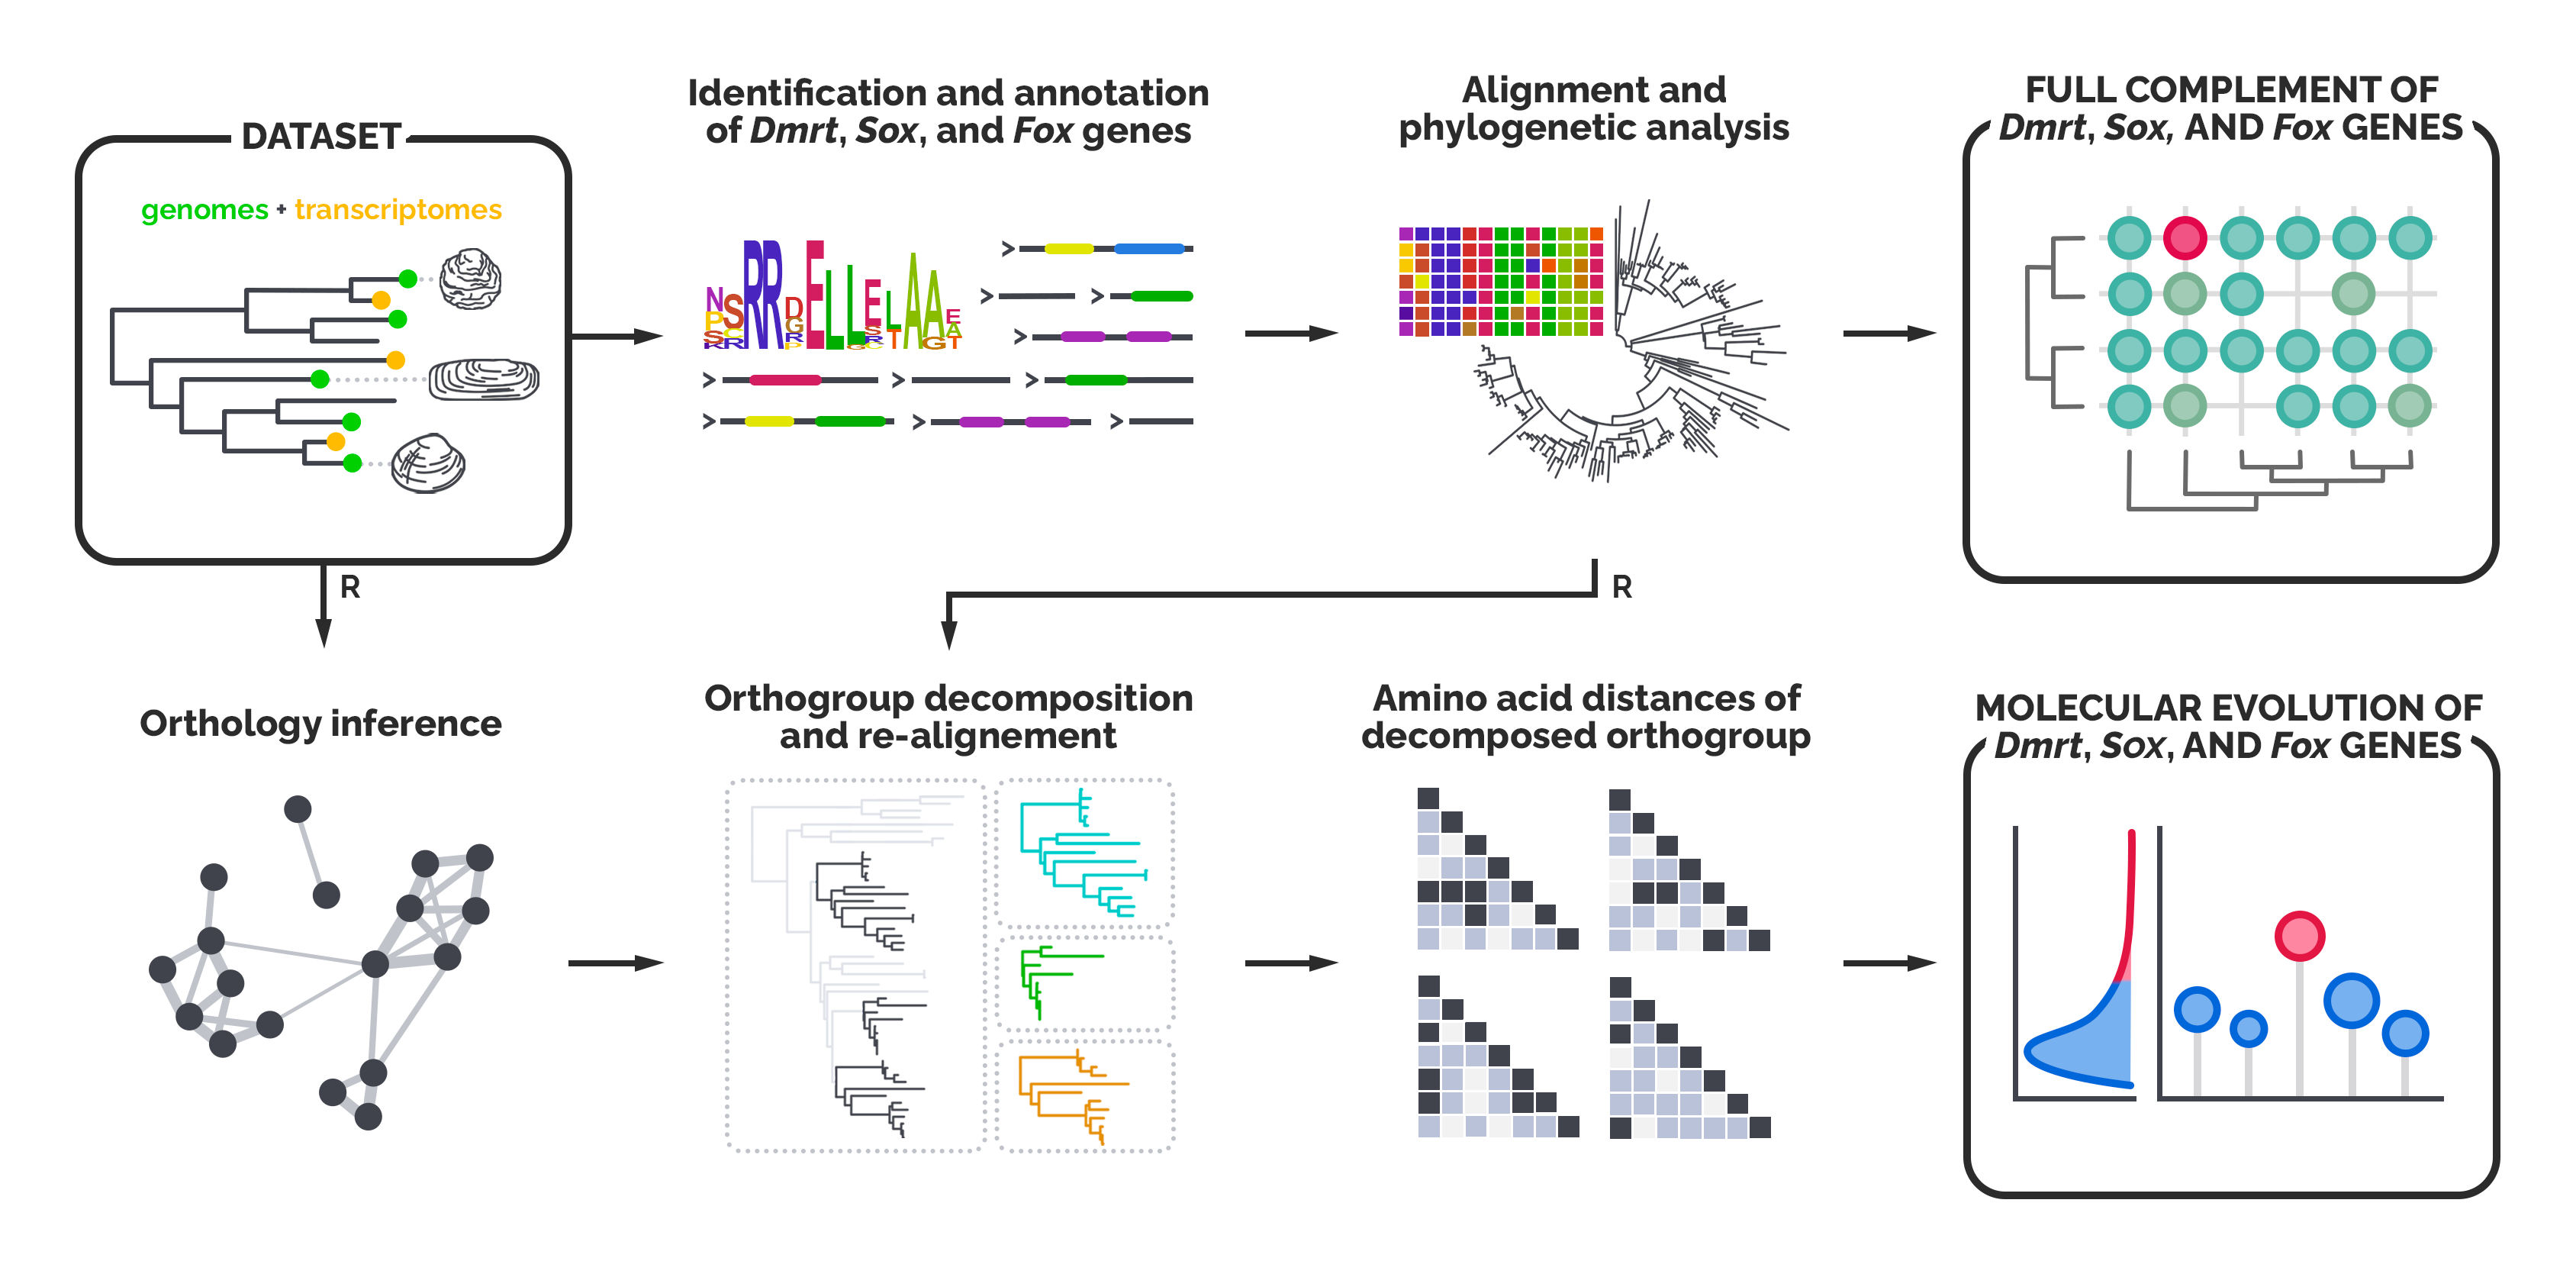
\includegraphics[width=\textwidth]{chapter3/figure_1.png}
	
	\caption[\textbf{Workflow of the analyses for the bivalve dataset}]
	{
		\textbf{Workflow of the analyses for the bivalve dataset}. Starting from a set of both genomes and transcriptomes covering a great portion of bivalve taxonomic diversity, we first characterized the entire complement of 	gls{dsfg} genes (upper row). In particular, we used sequence annotation and phylogenetic tools to obtain reliable sequences and filter out any putative mis-assembled or mis-annotated sequence. Afterwards, we built a reduced set of transcriptomes and genomes (the reduced bivalve dataset, where we minimized the redundancy of congeneric species) from which to draw the molecular evolution patterns of orthologous genes (bottom row). In particular, after having obtained gene single-copy orthologous groups, we calculated the amino acid distances within each orthogroup and then we built the distribution of median values. The same pipeline was also employed for the mammal and the fruit fly datasets, with just two minor differences: the starting dataset was composed of only genomes, and that the reduction step (R) was not necessary.
	}
	\label{fig:workflow}
\end{figure}

\subsection{GO-term enrichment}
After having obtained the distributions of \gls{aasd} in the three datasets (Bivalvia, Mammalia, and \textit{Drosophila}) and having sorted \glspl{sco} genes up into 3 groups (Group 1, Group 2, and Group 3), we performed a \gls{go} enrichment analysis of genes from Group 1 and genes from Group 1 + Group 2. To do so, we firstly selected one gene per SCO, giving priority to few chosen species: (i) for bivalves, we selected genes from Pecten maximus, or alternatively from \gls{cgig}, \gls{hbia} (now \textit{Unio delphinus}), \gls{tsqu}, and \gls{sgra}; (ii) for mammals, we selected genes from \gls{hsap}, or alternatively from \gls{bbub}, \gls{ptig}, \gls{cdro}, and \gls{mdom}; (iii) for fruit flies, we selected genes from \gls{dmel}, or alternatively from \gls{dhyd}, \gls{dpse}, and \gls{dsuz}. By doing so, we ensured that each \gls{sco} was represented by one gene. Afterwards, we annotated the obtained datasets with the corresponding \gls{go} terms using the OMA browser (accessed 18/09/2024; \textbf{\cite{altenhoff2024oma}}). The \gls{go}-term enrichment of Group 1 genes and Group 1 + Group 2 genes was performed with the R package ‘topGO’ with the Fisher exact test (\textbf{\cite{alexa2009gene}}).

\section{Results} \label{chapter3_results}
\subsection{Genomic and transcriptomic datasets}
The complete bivalve dataset consists of 29 bivalve genomes, 14 bivalve transcriptomes, and 7 outgroup genomes (5 gastropods and 2 \textit{Octopus} spp.; \cref{suppTab:bivalve_dataset}). BUSCO statistics for complete single-copy genes spanned from the 64.9\% in \gls{mmod} to the 99.4\% of \gls{pvir}, with a median value of 94.7\%. We were able to get at least one representative species for 11 different bivalve orders, covering a good proportion of the phylogenetic diversity of the clades Pteriomorphia, Palaeoheterodonta, and Imparidentia, and thus building the most extensive genomic and transcriptomic dataset for bivalve comparative analyses so far (\cref{suppTab:bivalve_dataset}). Unfortunately, no genomes or transcriptomes for Protobranchia, Archiheterodonta, and Anomalodesmata were available at the time of the project, thus we were not able to include any of those clades in our analysis. The reduced bivalve dataset (used for the orthology inference and the molecular evolution analysis; \cref{fig:workflow}) consists instead of 36 genomes and transcriptomes (\cref{suppTab:bivalve_dataset}), and was built to retain just one species for each taxonomic genera.

The mammal dataset consists of 32 species and 1 outgroup (\gls{ggal}, Aves; \cref{suppTab:mammal_dataset}), and covers 12 major orders, while the fruit fly dataset consists of 17 species and 1 outgroup (\gls{agam}, Culicidae; \cref{suppTab:drosophila_dataset}), and covers 2 \textit{Drosophila} subgenera (i.e., \textit{Drosophila} and \textit{Sophophora}). BUSCO statistics for complete single-copy genes were generally higher than those of bivalves, with a median of 98.3\% for mammals and of 99.8\% for fruit flies (\cref{suppTab:mammal_dataset,suppTab:drosophila_dataset}).

\subsection{The Dmrt, Sox, and Fox complements in bivalves}
Our annotation pipeline managed to successfully identify and annotate \glspl{dsfg} in bivalves, as proved by the same analysis in mammals and fruit flies (see the paragraph \textbf{The Dmrt, Sox, and Fox complements and their amino acid divergence in the testing datasets} COMPLETARE COMPLETARE).

We retrieved four main orthology groups of \gls{dmrt} genes in bivalves (\cref{fig:DSFG_bivalveCompilation,suppFig:dmrt_bivalves,suppTab:dsfg_bivalveAnnotation}), three corresponding to the groups present in the Bilateria common ancestor (\textit{Dmrt-2}, \textit{Dmrt-3}, and \textit{Dmrt-4/5}; \textbf{\cite{mawaribuchi2019independent}}), and one additional group with no unambiguous ortholog among reference genes, and thus putatively specific to molluscs (named \gls{dmrt-1l}, as per \textbf{\cite{li2018foxl2,evensen2022comparative}}). The majority of identified \gls{dmrt} genes are present in single-copy in each species, but \textit{Dmrt-4/5}s show a group-specific expansion in Palaeoheterodonta and Heterodonta, while \gls{dmrt-1l} is completely absent from Heterodonta. The degree of missing data for \gls{dmrt} genes in bivalves is about 35\%, with \textit{Dmrt-2} having the highest (about 56\%) and \textit{Dmrt-4/5} the lowest (about 7\%; \cref{suppTab:missing_data}). The \gls{cue}-like \gls{dma} domain has been annotated in most of the \textit{Dmrt-3} and \textit{Dmrt-4/5} genes, while an additional \gls{dm} domain has been annotated in \gls{dmrt-1l} genes in Mytilida and the gastropod \gls{pcan} (\cref{suppTab:dsfg_bivalveAnnotation}). Additionally, we retrieved six main orthology groups of \gls{sox} genes, none of which is restricted to molluscs or bivalves (\cref{fig:DSFG_bivalveCompilation,suppFig:sox_bivalves,suppTab:dsfg_bivalveAnnotation}). Five \gls{sox} groups (\textit{Sox-B1/2}, \textit{Sox-C}, \textit{Sox-D}, \textit{Sox-E}, and \textit{Sox-F}) are those traditionally considered to be present in the Bilateria common ancestor (\textbf{\cite{phochanukul2010no}}), while one has been identified outside mammals only recently (\textit{Sox-H}, or \textit{Sox-30}; \textbf{\cite{han2010characterization}}). \textit{Sox-B2} and \textit{Sox-B1} have been grouped in the same clade, as in our phylogenetic reconstruction the former results in a paraphyletic group with the latter (\cref{suppFig:sox_bivalves}), despite being traditionally recognised as a separate paralogy group in humans, fruit flies, and nematodes. The degree of missing data for \gls{sox} genes in bivalves is about 8\%, with \textit{Sox-H} having the highest (about 21\%) and \textit{Sox-B1/2} and \textit{Sox-C} both having no missing genes (\cref{suppTab:missing_data}). The \gls{sox} N-terminal signature domain was annotated for \textit{Sox-E} genes (\cref{suppTab:dsfg_bivalveAnnotation}). Concerning \gls{fox} genes, we retrieved 27 main orthology groups (\cref{fig:DSFG_bivalveCompilation,suppFig:fox_bivalves,suppTab:dsfg_bivalveAnnotation}), two of which are specific to molluscs (\textit{Fox-OG13/NA}, \textit{Fox-OG16/NA}). Additionally, other potential mollusc-specific \gls{fox} groups have been identified, but these have been excluded from the final orthology analysis as they are present in less than half of bivalve species (see \textbf{Materials and Methods} REFERENCE REFERENCE; \cref{suppTab:dsfg_bivalveAnnotation}). The two major \gls{fox} gene subgroups, Group I (monophyletic, specific to Metazoa; includes \textit{Fox-A}, \textit{Fox-B}, \textit{Fox-C}, \textit{Fox-D}, \textit{Fox-E}, \textit{Fox-F}, \textit{Fox-G}, \textit{Fox-H}, \textit{Fox-L1}, \textit{Fox-L2}, \textit{Fox-Q2}) and Group II (paraphyletic, specific to Opisthokonta; includes \textit{Fox-O}, \textit{Fox-P}, \textit{Fox-J2}, \textit{Fox-J1}, \textit{Fox-K}, \textit{Fox-N2/3}, \textit{Fox-N1/4}; \textbf{\cite{larroux2008genesis}}), have been recovered, including the four \gls{fox} genes that were present in the Bilateria common ancestor (\textit{Fox-C}, \textit{Fox-F}, \textit{Fox-L1}, and \textit{Fox-Q1}; \textbf{\cite{shimeld2010clustered}}). Two putative lineage-specific expansions have been recovered for \textit{Fox-OG28/NA}, one regarding \textit{Mytilus} spp. and one regarding the two Myida species (\cref{fig:DSFG_bivalveCompilation}; \cref{suppFig:fox_bivalves}). The degree of missing data for \gls{fox} genes in bivalves is about 22\%, with \textit{Fox-H} having the highest (about 42\%) and \textit{Fox-J1} having no missing genes (\cref{suppTab:missing_data}). The \gls{fha} domain was annotated for \textit{Fox-K} genes, the \textit{Fox-P} coiled-coil signature domain was annotated for \textit{Fox-P} genes, while both the forkhead N- and C-terminal signature domains were annotated for \textit{Fox-A} genes (\cref{suppTab:dsfg_bivalveAnnotation}).
Regarding bivalve species, the amount of missing data greatly differs between genomes and transcriptomes, with a mean of about 9\% and about 45\%, respectively. \gls{airc}, \textit{Mytilus unguiculatus} (formerly \textit{coruscus}), and \gls{pmax} have no missing data, while \gls{lorb} has the highest proportion (about 64\%; \cref{suppTab:missing_data}).


\begin{figure}
	\centering
	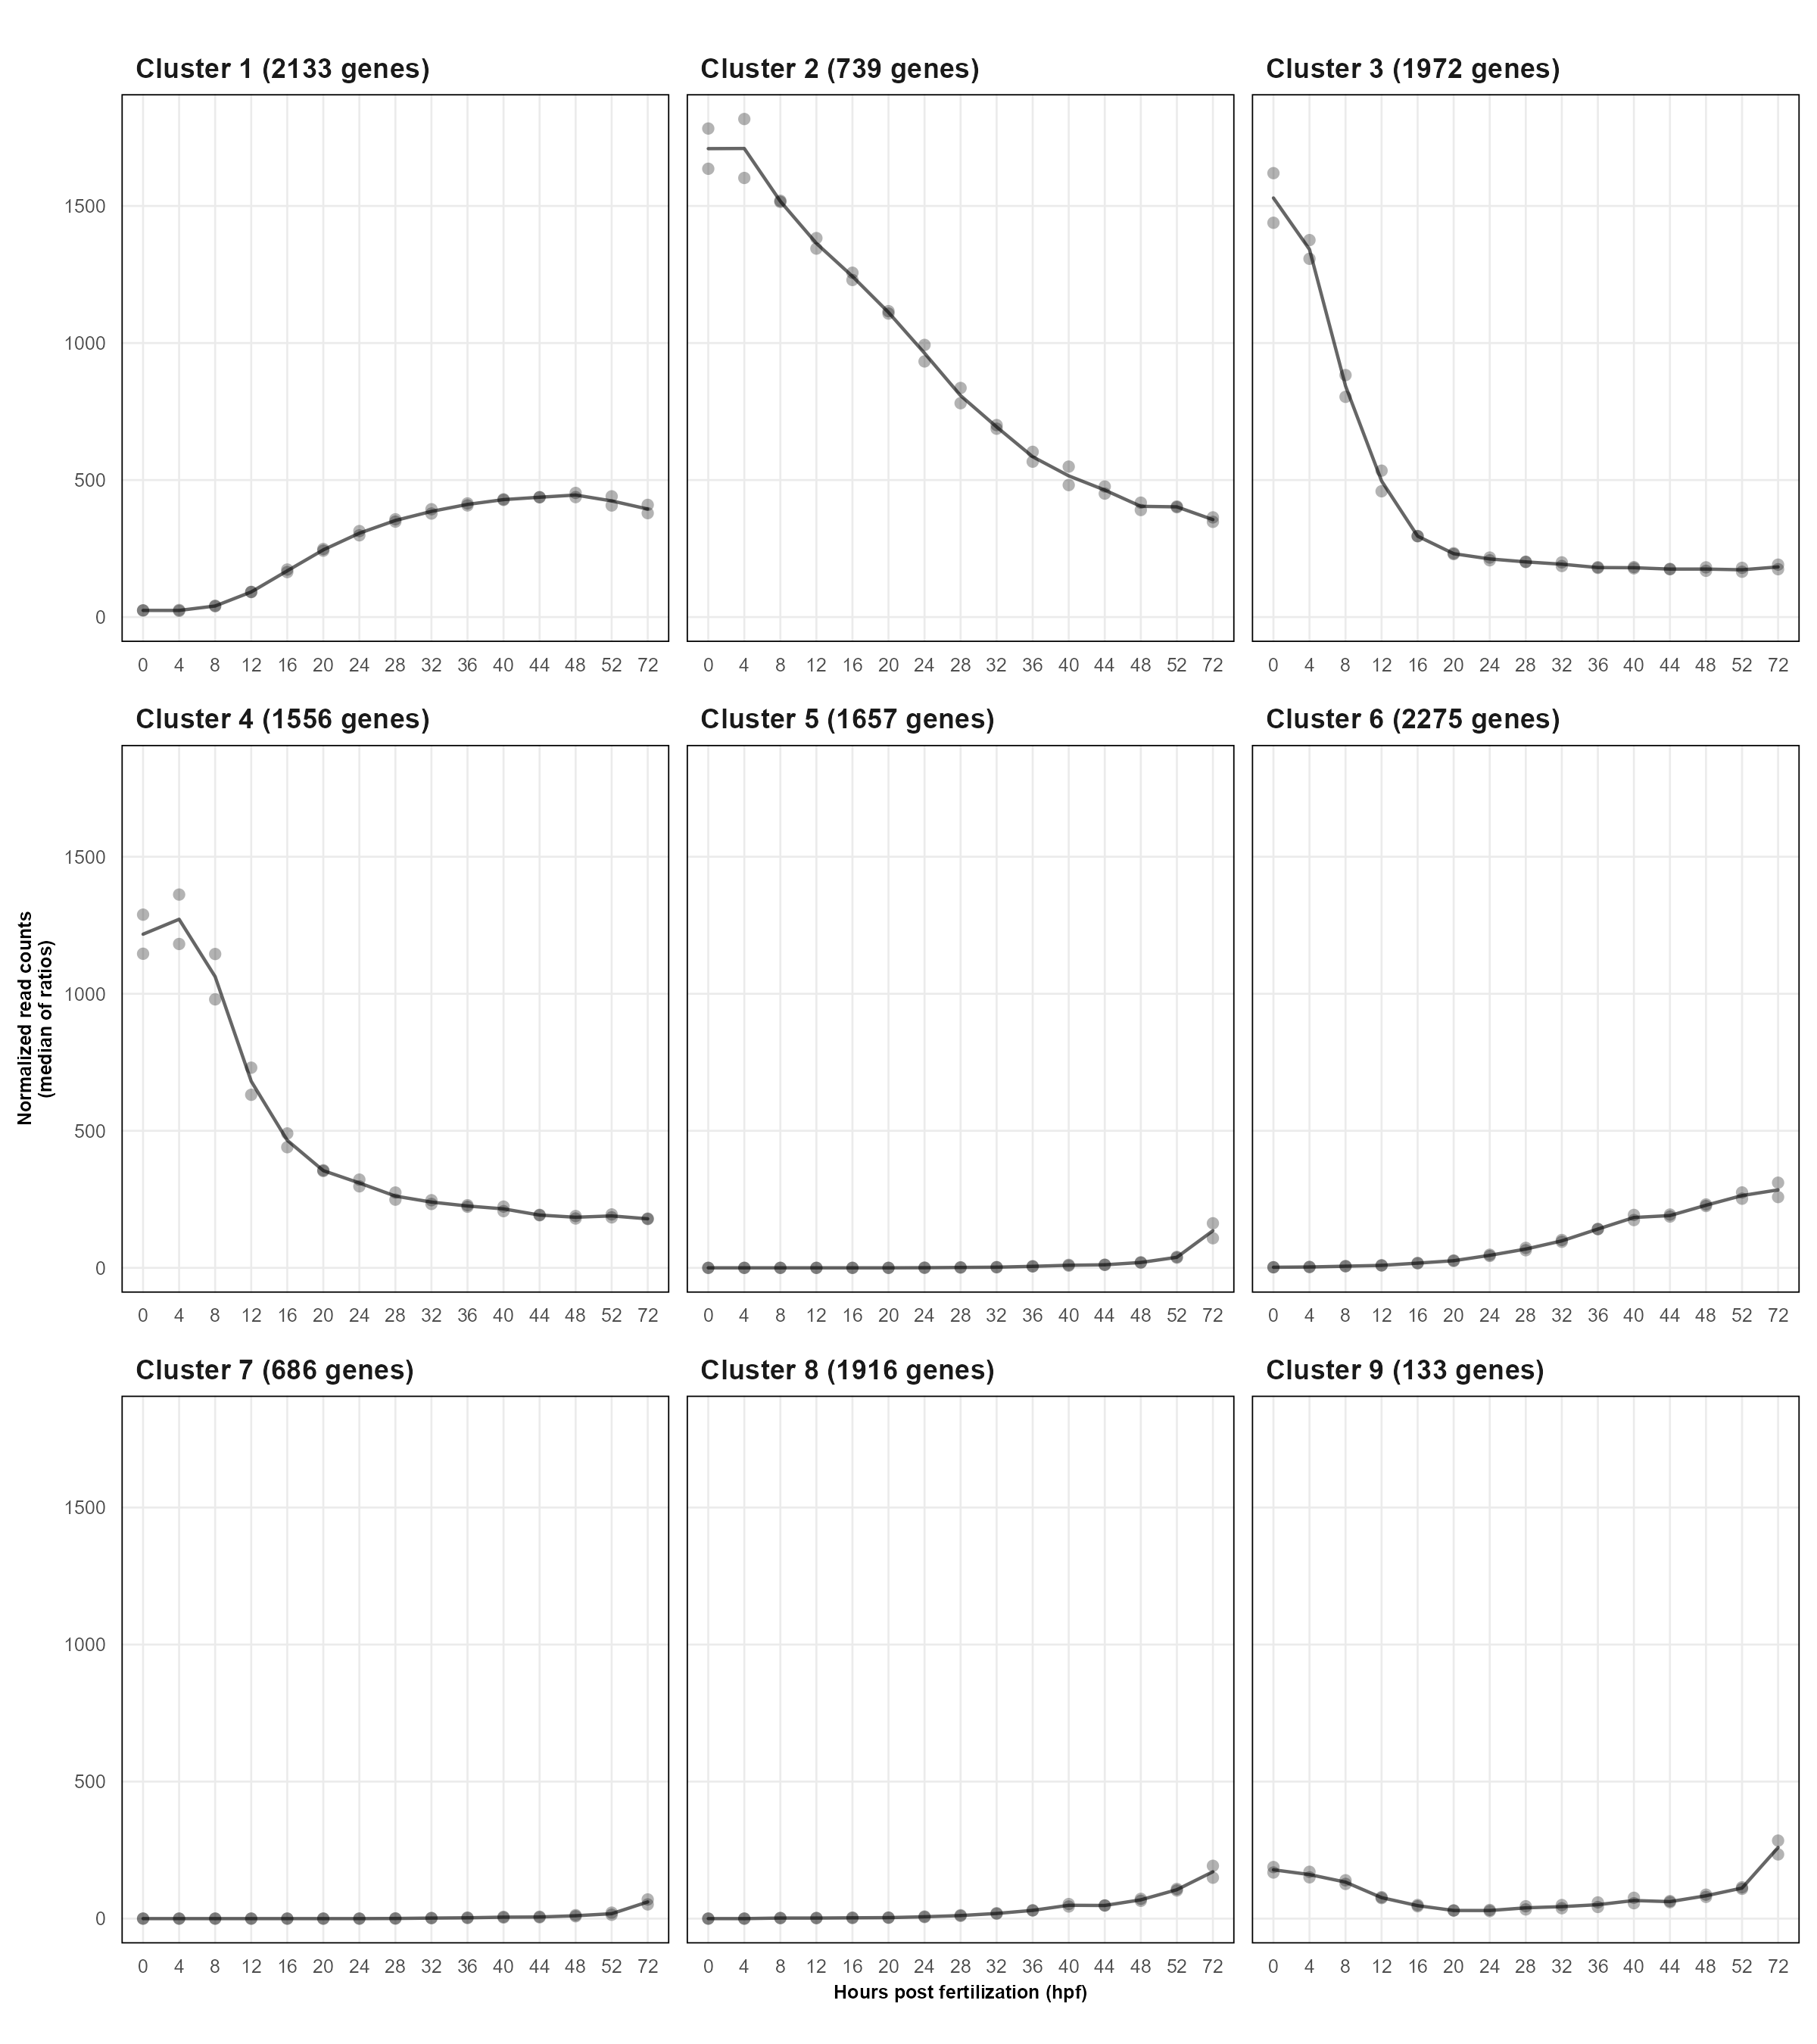
\includegraphics[width=\textwidth]{chapter3/figure_2.png}
	
	\caption[\textbf{\gls{dsfg} complement in bivalves and their outgroups}]
	{
		\textbf{\gls{dsfg} complement in bivalves and their outgroups}. Presence/absence of genes in various species are indicated by filled circles. Numbers inside each circle specify genes with 2 or more copies. The shaded area highlights non-bivalve species, belonging either to other molluscs or to the references. The phylogenetic tree of analyzed species, as inferred from literature, is shown on the left, while major taxonomic groups are reported on the right. Species represented by transcriptomic data are marked with an asterisk (‘*’), and species not present in the reduced bivalve dataset are marked with two asterisks (‘**’; see main text and \cref{fig:workflow}); note that the two categories do nor overlap. DSFG trees are shown on the bottom (full trees can be found in \cref{suppFig:dmrt_bivalves,suppFig:fox_bivalves}). Full species names, along with all assembly and taxonomic information, can be found in \cref{suppTab:bivalve_dataset}.  Ad.: Adapedonta; Ar.: Arcida; Ca.: Cardiida; Ce.: Cephalopoda; L.: Lucinida; My.: Myida; Ref.: reference genes; S.: Sphaeriida.
	}
	\label{fig:DSFG_bivalveCompilation}
\end{figure}

\subsection{Amino acid sequence divergence of Dmrt, Sox, and Fox genes in bivalves}
In the reduced bivalve dataset, OrthoFinder collectively analysed $>$1.2G genes distributed in 34 species. 89.4\% of these genes were placed in orthogroups, while 10.6\% were not. The number of retrieved \glspl{sco} is 5, which is drastically low but can be explained considering the mixed nature of the dataset, that is, it includes both genomes and transcriptomes with highly different BUSCO scores (\cref{suppTab:bivalve_dataset}). In order to be able to analyse a greater number of genes, we decomposed OrthoFinder orthogroups using DISCO and eventually obtained ~11k \glspl{sco} with at least 50\% of the species. By running the same pipeline on \glspl{dsfg}, we included in the \gls{aasd} analysis 32 \glspl{sco} (\cref{fig:DSFG_bivalveCompilation}) out of 33 initial Possvm-identified groups (\textit{Fox-H} didn’t meet the species occupancy threshold; \cref{fig:DSFG_bivalveDivergence}).

\begin{figure}
	\centering
	\includegraphics[width=\textwidth]{chapter3/figure_3.png}
	\captionsetup[subfigure]{labelformat=nocaption}
	\begin{subfigure}{0\linewidth}
	\caption{}\label{fig:DSFG_bivalveDivergence-A}
	\end{subfigure}% <----- get rid of space, for proper centering
	\begin{subfigure}{0\linewidth}
	\caption{}\label{fig:DSFG_bivalveDivergence-B}
	\end{subfigure}% <----- get rid of space, for proper centering
	\begin{subfigure}{0\linewidth}
	\caption{}\label{fig:DSFG_bivalveDivergence-C}
	\end{subfigure}% <----- get rid of space, for proper centering
	\begin{subfigure}{0\linewidth}
	\caption{}\label{fig:DSFG_bivalveDivergence-D}
	\end{subfigure}% <----- get rid of space, for proper centering
	\begin{subfigure}{0\linewidth}
	\caption{}\label{fig:DSFG_bivalveDivergence-E}
	\end{subfigure}
	
	\caption[\textbf{Distribution of \gls{aasd} of single-copy orthogroups in bivalves (A), including \glspl{dsfg} (B), and their correlations with tip-to-tip distances (C), alignment lengths (D), and number of species (E)}]
	{
		\textbf{Distribution of \gls{aasd} of single-copy orthogroups in bivalves (A), including \glspl{dsfg} (B), and their correlations with tip-to-tip distances (C), alignment lengths (D), and number of species (E)}. The distribution of AASD has been computed on the median values of pairwise distances of $>$11k \glspl{sco} from the reduced bivalve dataset (see main text and \cref{fig:workflow}). Genes have been divided according to their median \gls{aasd} value into three different groups, which are indicated by different colors and increasing numbers (Groups 1, 2, and 3). Circle heights of \glspl{dsfg} show the median value of their \gls{aasd}, while the size indicates the number of represented species. \gls{dsfg} trees are shown on the bottom (full trees can be found in \cref{suppFig:dmrt_bivalves,suppFig:fox_bivalves}). Darker points in C--E indicate \gls{dsfg} \glspl{sco}. The correlation between the amino acid distance and the tip-to-tip distance has been computed on 200 randomly-selected orthogroups.
	}
	\label{fig:DSFG_bivalveDivergence}
\end{figure}

From the distribution of median \gls{aasd}, 112 genes were assigned to Group 1 (1\% upper quantile), 447 to Group 2 (5\% upper quantile), and 10.603 to Group 3. Most of the \glspl{dsfg} (29/32) fell in Group 3 (\cref{fig:DSFG_bivalveDivergence}), which means they have a median \gls{aasd} comparable to the vast majority of other genes in bivalves (median level of the genomes). Just \gls{dmrt-1l}, \textit{Sox-H}, and \textit{Sox-F} showed higher divergences, and have been accordingly placed in Group 2. Overall, pairwise \gls{aasd} proved to be a good approximation of the tip-to-tip distances ($R = 0.84, p < \num{2.2e-16}$, calculated on 200 randomly-selected trees; \cref{fig:DSFG_bivalveDivergence}\textbf{C}), while it showed no influence from the alignment length ($R = 0.11$) or the number of represented species ($R = -0.23$; \cref{fig:DSFG_bivalveDivergence}\textbf{D--E}). Genes from Group 1 and Group 2 are strongly involved in cellular regulatory processes (such as those related to the metabolism of nucleic acids, proteins, and other macromolecules), but also in development and response to external stimuli, as shown by the GO-term enrichment analysis (\cref{tab:enrichedGOs,suppTab:enrichedGOs_complete}).

\begin{landscape}
	\footnotesize
	\begin{longtable}[c]{@{}lllccr@{}}
		\caption[\textbf{Top enriched GO terms for Group 1 and Group 2 genes of bivalves, mammals, and \textit{Drosophila}}]
		{
			\textbf{Top enriched GO terms for Group 1 and Group 2 genes of bivalves, mammals, and \textit{Drosophila}}. The extended version of the table, which includes also the expected number of annotated genes per GO term and all the other enriched GO terms, can be accessed in \cref{suppTab:enrichedGOs_complete}.
		}
		\label{tab:enrichedGOs}                                                                                                                                                                                                                                                                                                                                                                                \\
		\toprule
		\multicolumn{1}{c}{\textbf{Dataset}}           & \multicolumn{1}{c}{\textbf{GO.ID}} & \multicolumn{1}{c}{\textbf{Term}}                                         & \textbf{\begin{tabular}[c]{@{}c@{}}Annotated\\ genes\end{tabular}} & \textbf{\begin{tabular}[c]{@{}c@{}}Significant\\ genes\end{tabular}} & \multicolumn{1}{c}{\textbf{\begin{tabular}[c]{@{}c@{}}Corrected\\ p-value\end{tabular}}} \\* \midrule \midrule
		\endfirsthead
		%
		\multicolumn{6}{c}%
		{\textbf{Tab. \thetable} continued from previous page}                                                                                                                                                                                                                                                                                                                                             \\
		\toprule
		\multicolumn{1}{c}{\textbf{Dataset}}           & \multicolumn{1}{c}{\textbf{GO.ID}} & \multicolumn{1}{c}{\textbf{Term}}                                         & \textbf{\begin{tabular}[c]{@{}c@{}}Annotated\\ genes\end{tabular}} & \textbf{\begin{tabular}[c]{@{}c@{}}Significant\\ genes\end{tabular}} & \multicolumn{1}{c}{\textbf{\begin{tabular}[c]{@{}c@{}}Corrected\\ p-value\end{tabular}}} \\* \midrule \midrule
		\endhead
		%
		\endfoot
		%
		\endlastfoot
		%
		\multirow{21}{*}{\textbf{Bivalvia}}            & GO:0060255                         & regulation of macromolecule metabolic process                             & 737                                                                & 59                                                                   & 0.04525                                                                                  \\
		                                               & GO:0080090                         & regulation of primary metabolic process                                   & 673                                                                & 53                                                                   & 0.01818                                                                                  \\
		                                               & GO:0019219                         & regulation of nucleobase-containing compound metabolic process            & 541                                                                & 41                                                                   & 0.02388                                                                                  \\
		                                               & GO:0006351                         & DNA-templated transcription                                               & 571                                                                & 39                                                                   & 0.03767                                                                                  \\
		                                               & GO:0032774                         & RNA biosynthetic process                                                  & 579                                                                & 39                                                                   & 0.04490                                                                                  \\
		                                               & GO:0051252                         & regulation of RNA metabolic process                                       & 517                                                                & 37                                                                   & 0.02719                                                                                  \\
		                                               & GO:0006355                         & regulation of DNA-templated transcription                                 & 490                                                                & 35                                                                   & 0.03751                                                                                  \\
		                                               & GO:2001141                         & regulation of RNA biosynthetic process                                    & 491                                                                & 35                                                                   & 0.03844                                                                                  \\
		                                               & GO:0006950                         & response to stress                                                        & 370                                                                & 33                                                                   & 0.01949                                                                                  \\
		                                               & GO:0032502                         & developmental process                                                     & 261                                                                & 27                                                                   & 0.04445                                                                                  \\
		                                               & GO:0006468                         & protein phosphorylation                                                   & 345                                                                & 23                                                                   & 0.02483                                                                                  \\
		                                               & GO:0031325                         & positive regulation of cellular metabolic process                         & 125                                                                & 17                                                                   & 0.00801                                                                                  \\
		                                               & GO:0010604                         & positive regulation of macromolecule metabolic process                    & 151                                                                & 17                                                                   & 0.04047                                                                                  \\
		                                               & GO:0051172                         & negative regulation of nitrogen compound metabolic process                & 117                                                                & 16                                                                   & 0.00814                                                                                  \\
		                                               & GO:0051173                         & positive regulation of nitrogen compound metabolic process                & 137                                                                & 15                                                                   & 0.02454                                                                                  \\
		                                               & GO:0006310                         & DNA recombination                                                         & 66                                                                 & 14                                                                   & 0.00087                                                                                  \\
		                                               & GO:0048513                         & animal organ development                                                  & 83                                                                 & 12                                                                   & 0.04088                                                                                  \\
		                                               & GO:0010629                         & negative regulation of gene expression                                    & 78                                                                 & 11                                                                   & 0.00048                                                                                  \\
		                                               & GO:0023051                         & regulation of signaling                                                   & 133                                                                & 11                                                                   & 0.02872                                                                                  \\
		                                               & GO:0045934                         & negative regulation of nucleobase-containing compound metabolic process   & 64                                                                 & 11                                                                   & 0.03637                                                                                  \\
		                                               & GO:0009605                         & response to external stimulus                                             & 90                                                                 & 11                                                                   & 0.04544                                                                                  \\
		\multirow{1}{*}{\textbf{Bivalvia}}             & GO:0044419                         & biological process involved in interspecies interaction between organisms & 63                                                                 & 11                                                                   & 0.04761                                                                                  \\* \midrule
		\multirow{22}{*}{\textbf{Mammalia}}            & GO:0006955                         & immune response                                                           & 1297                                                               & 145                                                                  & 0.00061                                                                                  \\
		                                               & GO:0098542                         & defense response to other organism                                        & 853                                                                & 112                                                                  & 0.02066                                                                                  \\
		                                               & GO:0045087                         & innate immune response                                                    & 647                                                                & 82                                                                   & 8.5e-10                                                                                  \\
		                                               & GO:0001817                         & regulation of cytokine production                                         & 630                                                                & 51                                                                   & 0.04660                                                                                  \\
		                                               & GO:0042742                         & defense response to bacterium                                             & 233                                                                & 45                                                                   & 1.7e-07                                                                                  \\
		                                               & GO:0006954                         & inflammatory response                                                     & 642                                                                & 45                                                                   & 0.01735                                                                                  \\
		                                               & GO:0019221                         & cytokine-mediated signaling pathway                                       & 382                                                                & 44                                                                   & 3.9e-07                                                                                  \\
		                                               & GO:0002250                         & adaptive immune response                                                  & 342                                                                & 44                                                                   & 1.3e-05                                                                                  \\
		                                               & GO:0001819                         & positive regulation of cytokine production                                & 402                                                                & 41                                                                   & 0.02723                                                                                  \\
		                                               & GO:0002697                         & regulation of immune effector process                                     & 308                                                                & 37                                                                   & 0.04426                                                                                  \\
		                                               & GO:0042110                         & T cell activation                                                         & 432                                                                & 35                                                                   & 0.02564                                                                                  \\
		                                               & GO:0051607                         & defense response to virus                                                 & 257                                                                & 34                                                                   & 1.9e-07                                                                                  \\
		                                               & GO:0048232                         & male gamete generation                                                    & 491                                                                & 32                                                                   & 0.02255                                                                                  \\
		                                               & GO:0007283                         & spermatogenesis                                                           & 478                                                                & 31                                                                   & 0.02801                                                                                  \\
		                                               & GO:0070661                         & leukocyte proliferation                                                   & 273                                                                & 29                                                                   & 0.01285                                                                                  \\
		                                               & GO:0002449                         & lymphocyte mediated immunity                                              & 221                                                                & 29                                                                   & 0.04833                                                                                  \\
		                                               & GO:0070663                         & regulation of leukocyte proliferation                                     & 212                                                                & 25                                                                   & 0.01870                                                                                  \\
		                                               & GO:0050727                         & regulation of inflammatory response                                       & 300                                                                & 24                                                                   & 0.00235                                                                                  \\
		                                               & GO:0031349                         & positive regulation of defense response                                   & 240                                                                & 24                                                                   & 0.01239                                                                                  \\
		                                               & GO:0002768                         & immune response-regulating cell surface receptor signaling pathway        & 177                                                                & 22                                                                   & 0.00336                                                                                  \\
		                                               & GO:0050829                         & defense response to Gram-negative bacterium                               & 66                                                                 & 17                                                                   & 1.7e-10                                                                                  \\
		                                               & GO:0071222                         & cellular response to lipopolysaccharide                                   & 164                                                                & 17                                                                   & 0.00012                                                                                  \\
		\multirow{13}{*}{\textbf{Mammalia}}            & GO:0010466                         & negative regulation of peptidase activity                                 & 163                                                                & 16                                                                   & 0.00036                                                                                  \\
		                                               & GO:0002429                         & immune response-activating cell surface receptor signaling pathway        & 164                                                                & 16                                                                   & 0.00243                                                                                  \\
		                                               & GO:1903555                         & regulation of tumor necrosis factor superfamily cytokine production       & 137                                                                & 16                                                                   & 0.01244                                                                                  \\
		                                               & GO:0071706                         & tumor necrosis factor superfamily cytokine production                     & 137                                                                & 16                                                                   & 0.01244                                                                                  \\
		                                               & GO:0070665                         & positive regulation of leukocyte proliferation                            & 132                                                                & 16                                                                   & 0.02765                                                                                  \\
		                                               & GO:0045089                         & positive regulation of innate immune response                             & 113                                                                & 16                                                                   & 0.03224                                                                                  \\
		                                               & GO:0071356                         & cellular response to tumor necrosis factor                                & 175                                                                & 15                                                                   & 0.00219                                                                                  \\
		                                               & GO:0002695                         & negative regulation of leukocyte activation                               & 148                                                                & 15                                                                   & 0.01151                                                                                  \\
		                                               & GO:0002456                         & T cell mediated immunity                                                  & 82                                                                 & 15                                                                   & 0.01605                                                                                  \\
		                                               & GO:0002705                         & positive regulation of leukocyte mediated immunity                        & 113                                                                & 15                                                                   & 0.01837                                                                                  \\
		                                               & GO:0032680                         & regulation of tumor necrosis factor production                            & 133                                                                & 15                                                                   & 0.03262                                                                                  \\
		                                               & GO:0032640                         & tumor necrosis factor production                                          & 133                                                                & 15                                                                   & 0.03262                                                                                  \\
		                                               & GO:0050866                         & negative regulation of cell activation                                    & 165                                                                & 15                                                                   & 0.04048                                                                                  \\* \midrule
		\multirow{10}{*}{\textit{\textbf{Drosophila}}} & GO:0000819                         & sister chromatid segregation                                              & 140                                                                & 11                                                                   & 0.02927                                                                                  \\
		                                               & GO:0070192                         & chromosome organization involved in meiotic cell cycle                    & 54                                                                 & 9                                                                    & 0.00849                                                                                  \\
		                                               & GO:0007131                         & reciprocal meiotic recombination                                          & 37                                                                 & 7                                                                    & 0.00066                                                                                  \\
		                                               & GO:0007143                         & female meiotic nuclear division                                           & 54                                                                 & 6                                                                    & 0.02270                                                                                  \\
		                                               & GO:0035967                         & cellular response to topologically incorrect protein                      & 44                                                                 & 5                                                                    & 0.03334                                                                                  \\
		                                               & GO:0035966                         & response to topologically incorrect protein                               & 47                                                                 & 5                                                                    & 0.04266                                                                                  \\
		                                               & GO:0007141                         & male meiosis I                                                            & 13                                                                 & 4                                                                    & 0.00150                                                                                  \\
		                                               & GO:0140543                         & positive regulation of piRNA transcription                                & 3                                                                  & 3                                                                    & 6.9e-05                                                                                  \\
		                                               & GO:0010526                         & retrotransposon silencing                                                 & 8                                                                  & 3                                                                    & 0.00331                                                                                  \\
		                                               & GO:0007130                         & synaptonemal complex assembly                                             & 10                                                                 & 3                                                                    & 0.00666                                                                                  \\
		\multirow{5}{*}{\textit{\textbf{Drosophila}}}  & GO:0030719                         & P granule organization                                                    & 11                                                                 & 3                                                                    & 0.00888                                                                                  \\
		                                               & GO:0071218                         & cellular response to misfolded protein                                    & 12                                                                 & 3                                                                    & 0.01149                                                                                  \\
		                                               & GO:0051788                         & response to misfolded protein                                             & 12                                                                 & 3                                                                    & 0.01149                                                                                  \\
		                                               & GO:0007135                         & meiosis II                                                                & 15                                                                 & 3                                                                    & 0.02169                                                                                  \\
		                                               & GO:0034508                         & centromere complex assembly                                               & 19                                                                 & 3                                                                    & 0.04094                                                                                  \\* \bottomrule \bottomrule
	\end{longtable}
\end{landscape}

\subsection{Dmrt, Sox, and Fox genes, and amino acid sequence divergence in the test datasets}
The \gls{dsfg} datasets retrieved in mammals and fruit flies are far more complete than those in bivalves, and most of the already-recognised orthology groups have been identified.

In mammals, we retrieved 7 \gls{dmrt} orthology groups with about 3.1\% of missing data, 20 \gls{sox} orthology groups with about 8.1\% of missing data, and 42 \gls{fox} orthology groups with about 4.6\% of missing data (\cref{suppFig:DSFG_testCompilation-A}, \cref{suppFig:dmrt_mammals,suppFig:fox_mammals,suppTab:dsfg_mammalAnnotation}). Of these, just \textit{Sox-5} was not included in the subsequent \gls{aasd} analysis, as it did not meet the 50\%-species occupancy threshold. OrthoFinder analysed about 650M genes, and the number of \glspl{sco} used in the \gls{aasd} analysis (thus resulting from the DISCO-based orthogroup decomposition pipeline) is $>$16k (\cref{fig:DSFG_testDivergence-A}). From the distribution of median \gls{aasd}, 163 genes were assigned to Group 1, 649 to Group 2, and 15.355 to Group 3. Most of the \glspl{dsfg} (66/68) fell in Group 3 (\cref{fig:DSFG_testDivergence-B}), while \gls{sry} and \textit{Fox-D4} showed higher divergences, and have been accordingly placed in Group 1 and 2, respectively. Genes from Group 1 and Group 2 show a strong enrichment in immune-related functions (such as innate and adaptive immune response, defence response to bacteria and viruses, lymphocyte methabolism, etc.), but also in reproductive processes (such as spermatogenesis; \cref{tab:enrichedGOs,suppTab:enrichedGOs_complete}).

Concerning \textit{Drosophila}, we retrieved 4 \gls{dmrt} orthology groups with about 1.7\% of missing data, 7 \gls{sox} orthology groups with about 3.9\% of missing data, and 17 \gls{fox} genes with about 8.3\% of missing data (\cref{suppFig:DSFG_testCompilation-B,suppFig:dmrt_drosophila,suppFig:fox_drosophila,suppTab:dsfg_drosophilaAnnotation}). OrthoFinder analysed about 240M, and the distribution of median \gls{aasd} was built after $>$12k \glspl{sco} (\cref{fig:DSFG_testDivergence-C}). 126 genes were assigned to Group 1, 501 to Group 2, and 11.880 to Group 3. All of the \glspl{dsfg} have been used in the \gls{aasd} analysis, but none of them have been placed in Group 1 or 2, that is, all the \glspl{dsfg} in \textit{Drosophila} have an \gls{aasd} comparable to the median level of the genome (\cref{fig:DSFG_testDivergence-D}). Genes of Group 1 and Group 2 show a GO-term enrichment in meiotic processes, such as chromosome/chromatid organisation, and retrotransposon silencing (\cref{tab:enrichedGOs,suppTab:enrichedGOs_complete}).

\begin{figure}
	\centering
	\includegraphics[width=0.9\textwidth]{chapter3/figure_4.png}
	\captionsetup[subfigure]{labelformat=nocaption}
	\begin{subfigure}{0\linewidth}
	\caption{}\label{fig:DSFG_testDivergence-A}
	\end{subfigure}% <----- get rid of space, for proper centering
	\begin{subfigure}{0\linewidth}
	\caption{}\label{fig:DSFG_testDivergence-B}
	\end{subfigure}% <----- get rid of space, for proper centering
	\begin{subfigure}{0\linewidth}
	\caption{}\label{fig:DSFG_testDivergence-C}
	\end{subfigure}% <----- get rid of space, for proper centering
	\begin{subfigure}{0\linewidth}
	\caption{}\label{fig:DSFG_testDivergence-D}
	\end{subfigure}
	
	\caption[\textbf{Distribution of \gls{aasd} of single-copy orthogroups in Mammalia (A) and \textit{Drosophila} (C), including \gls{dsfg} (B-D)}]
	{
		\textbf{Distribution of \gls{aasd} of single-copy orthogroups in Mammalia (A) and \textit{Drosophila} (C), including \gls{dsfg} (B-D)}. The distributions of AASD in mammals and fruit flies have been computed on the median values of pairwise distances of over 16k and 12k SCOs, respectively. Genes have been divided according to their median AASD value into three different groups, which are indicated by different colors and increasing numbers (Groups 1, 2, and 3). Circle heights of DSFGs show the median value of their AASD, while the size indicates the number of represented species. DSFG trees are shown on the bottom (full trees can be found in \cref{suppFig:dmrt_mammals,suppFig:sox_mammals,suppFig:fox_mammals} for mammals and in \cref{suppFig:dmrt_drosophila,suppFig:sox_drosophila,suppFig:fox_drosophila} for fruit flies). Insets: scheme of the sex-determination molecular pathways in \textit{Mus musculus} and in \textit{Drosophila melanogaster}, with shown the main genes involved (adapted from \textbf{\cite{beukeboom2014evolution}}). Green arrows indicate transcription activations, red arrows indicate transcription suppressions. X: sex chromosomes; A: autosomal chromosomes; \textit{DSX\textsuperscript{M/F}}: \textit{DSX} splicing variants present in males or females, respectively.
	}
	\label{fig:DSFG_testDivergence}
\end{figure}

\section{Discussion} \label{chpater3_discussion}
\subsection{A new manually-curated and phylogenetic-based reference dataset of Dmrt, Sox, and Fox genes in bivalves}
The annotation and characterisation process of a gene family in a certain clade of organisms may harbour many overlooked challenges (\textbf{\cite{vizueta2020bitacora}}). For example, the presence of highly-conserved catalytic domains may hamper the correct identification of the components of a gene family because of insufficient phylogenetic signal, as it is the case for Hox and ParaHox genes and their homeobox motif (\textbf{\cite{baldwin2018new, nicolini2023comparative}}). Conversely, the components of dynamic gene families characterised by abrupt and sequential duplication events may be difficult to sort into separate groups. As a matter of fact, varying levels of sequence heterogeneity and gene copy numbers makes the inference of orthologous groups hard, as for certain clans of the P450 gene family (\textbf{\cite{dermauw2020diversity}}). Regardless of the causes, having a solid and wide phylogenetic context in which to study gene duplications and losses, and orthology relationships, is crucial to overcome these difficulties. In the same way, manual curation and visual inspection of multiple sequence alignments, phylogenetic trees, and gene structures (in terms of domain annotation, start and stop codons, and other feature representations) is helpful, despite being time-demanding and possibly low reproducible. In this study, we characterised the full complement of \glspl{dsfg} in the vast class of bivalves, by leveraging sequence domain annotation, phylogenetics, and manual curation of the dataset. Our aim was to obtain the most reliable gene complements as possible, combined with a vast taxonomic dataset, a solid phylogenetic inference, an openly-available dataset of gene sequences, and a reproducible pipeline for the annotation of gene identity. By doing so, we want to provide a reliable resource for future studies of \glspl{dsfg}, either focused on bivalves or generally in Metazoa.

Concerning the \gls{dmrt} gene family, we identified orthologs of the vertebrate \textit{Dmrt-2}, \textit{Dmrt-3}, and \textit{Dmrt-4/5} (or \textit{A1/A2}; \cref{fig:DSFG_bivalveCompilation,suppFig:dmrt_bivalves,suppTab:dsfg_bivalveAnnotation}), which are also expected to have been present in the Bilateria common ancestor (\textbf{\cite{mawaribuchi2019independent}}). \textbf{\cite{wang2023genome}} found that \textit{Dmrt-4/5} is duplicated in \gls{mmer} and \gls{csin} (Venerida), and in \gls{dpol} (Myida), and we confirm this result by tracing back the duplication event to the split between Palaeoheterdonta (here represented by Unionida) and Heterodonta (here represented by Venerida, Myida, Sphaeriida, Adapedonta, Cardiida, and Lucinida; \cref{fig:DSFG_bivalveCompilation}). Furthermore, we confirm \gls{dmrt-1l} to be present in many bivalve species (mainly belonging to the Ostreida, Pectinida, Mytilida, and Unionida orders; \cref{fig:DSFG_bivalveCompilation}), as well as in gastropods and \textit{Octopus}. Though, our phylogenetic analysis did not retrieve any unambiguous orthology relationship among \gls{dmrt-1l} and either vertebrate \textit{Dmrt-1} or \textit{Drosophila} \gls{dsx} genes, as instead it was proposed in previous works (\textbf{\cite{li2018foxl2,evensen2022comparative}}). As a matter of fact, the amino acid sequence of the \gls{dmrt-1l} \gls{dm} domain does not recall that of any other \gls{dmrt} gene. Furthermore, it must be considered that various phylogenetic analyses have recovered both \textit{Dmrt-1} and \gls{dsx} genes to be restricted to vertebrates and arthropods, respectively (\textbf{\cite{wexler2014pan,mawaribuchi2019independent,panara2019phylogenetic}}), that is, they do not have any direct ortholog outside their relative clades. Thus, if \gls{dmrt-1l}, \gls{dsx}, and \textit{Dmrt-1} are true orthologs, their origin would need to be placed at least in the Bilateria common ancestor, which seems however to be not the case. All considered, we thus confirm that \gls{dmrt-1l} is not orthologous to \textit{Dmrt-1} and \gls{dsx} and is rather a mollusc-specific gene (\textbf{\cite{evensen2022comparative}}). The monophyly of the group is not supported by the phylogenetic tree inferred with \gls{dmrt} genes from molluscs and the reference species (\cref{suppFig:dmrt_bivalves}); though, it is recovered when analysing just genes from mollusc species (\cref{suppFig:dmrt_molluscOnly}). To this regard, we speculate that in our analysis, the difficulty in obtaining the monophyly of \gls{dmrt-1l} genes may have arisen primarily because of the many \gls{cele}-restricted genes (\cref{suppTab:reference_dsfgs}), which are placed among the other bivalve genes (\cref{suppFig:dmrt_bivalves}), but also because of the high \gls{aasd} of \gls{dmrt-1l} genes (see the following section), which hampers a straight-forward phylogenetic reconstruction. Furthermore, our broad-context analysis allowed us to identify some cases of incorrect gene identification in bivalves, which have arisen because of erroneous or ambiguous annotations in previous works, as a result of limited datasets or analyses. For example, (i) the scallop-specific cluster of \gls{dmrt} genes retrieved by \textbf{\cite{wang2023genome}} rather belongs to the \gls{dmrt-1l} group, and (ii) the classification of \gls{dmrt} genes in Crassostrea species provided by \textbf{\cite{zeng2024genome}} needs to be revised following the one of this work: \textit{Dmrt-1} genes are \textit{Dmrt-4/5}; \textit{Dmrt-2} genes are \textit{Dmrt-3}; \textit{Dmrt-3} genes are \gls{dmrt-1l}; hence, \textit{Crassostrea} species do not have \textit{Dmrt-2} genes.

For what concerns the \gls{sox} gene family, bivalves (or molluscs) do not show any major clade-restricted gene, as only the five Bilateria-specific \gls{sox} groups (\textit{Sox-B1/2}, \textit{Sox-C}, \textit{Sox-D}, \textit{Sox-E}, and \textit{Sox-F}) and \textit{Sox-H} have been identified (\cref{fig:DSFG_bivalveCompilation,suppFig:sox_bivalves.suppTab:dsfg_bivalveAnnotation}), in accordance with previous findings (\textbf{\cite{yu2017genome,evensen2022comparative, wang2024genome}}). \textit{Sox-B1/2} is clearly made up of two subgroups (i.e., \textit{Sox-B1} and \textit{Sox-B2}), as expected, but their respective identity could not be unambiguously established, as \textit{Sox-B1/2} genes of reference species do not form separate clusters (\cref{suppFig:sox_bivalves}). Even when inferring the phylogenetic tree only of components of the \textit{Sox-B1/2} group from molluscs and reference species, the identity can not be properly established (\cref{suppFig:sox_B12}).

Compared to \gls{dmrt} and \gls{sox} genes, the \gls{fox} gene family appears as the most dynamic in terms of gene presence/absence, as already shown by other works (\textbf{\cite{wu2020identification, seudre2022fox, schomburg2022phylogenetic}}). Our phylogenetic analysis successfully recovered Group I and Group II of \gls{fox} genes (\textbf{\cite{larroux2008genesis}}), which include the four \gls{fox} genes that were present in the Bilateria common ancestor (\textit{Fox-C}, \textit{Fox-F}, \textit{Fox-L1}, and \textit{Fox-Q1}; \cref{fig:DSFG_bivalveCompilation,suppFig:fox_bivalves,suppTab:dsfg_bivalveAnnotation}; \cite{shimeld2010clustered}). To our knowledge, this is the first broad-taxonomic identification and classification of \gls{fox} genes in bivalves, as up to now they have been systematically characterised only in \gls{cgig} (\textbf{\cite{yang2014phylogeny}}), \gls{pyes} (now \textit{Mizuhopecten yessoensis}; \textbf{\cite{wu2020identification}}), and \gls{rphi} (\textbf{\cite{liu2024characterization}}). Firstly, our analysis confirms the absence in molluscs of \textit{Fox-I}, \textit{Fox-Q1}, \textit{Fox-R}, \textit{Fox-S} (\cref{suppFig:fox_bivalves}), which are in fact thought to have emerged with the diversification of deuterostomes or vertebrates (\textbf{\cite{yang2014phylogeny, wu2020identification, seudre2022fox, schomburg2022phylogenetic}}). Furthermore, we have found many \gls{fox} groups that appeared as mollusc-specific and/or still-unnamed at a first analysis. However, a more in-depth investigation revealed a different scenario. \textit{Fox-OG2/NA} appears close to the human \textit{Fox-M} gene in the phylogenetic tree, but they do not form a monophyletic group (\cref{suppFig:fox_bivalves}). However, by comparing \textit{Fox-OG2/NA} sequences and phylogenetic tree with those analysed by \textbf{\cite{yang2014phylogeny}}, \textbf{\cite{wu2020identification}}, \textbf{\cite{schomburg2022phylogenetic}}, and \textbf{\cite{seudre2022fox}}, it appears clear that this group of \gls{fox} genes is indeed \textbf{Fox-M}. However, our analysis has failed to retrieve a monophyletic relationship among bivalve and human \textit{Fox-M} genes, even when inferring a tree with just \textit{Fox-J2}, \textit{Fox-M}, \textit{Fox-O}, and \textit{Fox-P} complements (\cref{suppFig:fox_JMOP}), which belong to the same \gls{fox} group. Regarding the \textit{Fox-OG39/NA} group, it does not have any homolog in reference species (\cref{suppFig:fox_bivalves}) but is found to belong to the \textit{Fox-AB} group by sequence comparison with previous works (\textbf{\cite{yang2014phylogeny, wu2020identification, seudre2022fox}}). \textit{Fox-AB} was formerly described only in the sea urchin \gls{spur} and the lancelet \gls{bflo} (\textbf{\cite{tu2006sea,yu2008fox}}), but was later identified also in several Spiralia lineages, including molluscs (e.g., \textbf{\cite{yang2014phylogeny, wu2020identification, seudre2022fox}}). A similar situation concerns \textit{Fox-OG15/NA} and \textit{Fox-OG28/NA}, which again could not be named based on orthology relationships with the reference species genes (\cref{suppFig:fox_bivalves}), but actually represent two lineage-specific expansions of the \textit{Fox-Q2} group (named \textit{Fox-Q2b} and \textit{Fox-Q2c}), as already appointed in previous studies (\textbf{\cite{yang2014phylogeny, wu2020identification}}). This observation fits within the wider context of the \textit{Fox-Q2} group expansion in Bilateria and, particularly, in Spiralia, that led to remarkable differences in their gene copy numbers across various clades (\textbf{\cite{seudre2022fox}}). Two additional \gls{fox} genes have been previously identified in bivalves, and were named \textit{Sox-Y} and \textit{Sox-Z} (\textbf{\cite{yang2014phylogeny, wu2020identification}}). In our analysis, these \gls{fox} groups were identified as \textit{Fox-OG13/NA} and \textit{Fox-OG16/NA}, after sequence comparison of \gls{fox} genes from \gls{cgig} and \gls{pyes}. On one hand, \textit{Fox-Y} was firstly identified in \gls{spur} (\textbf{\cite{tu2006sea}}) and only recently in a few bivalve species (\textbf{\cite{yang2014phylogeny, wu2020identification}}). However, when analysing bivalve and \gls{spur} \gls{fox} genes, we failed in retrieving such a clear orthology relationship, as \gls{spur} \textit{Fox-Y} does not fall within the phylogenetic range of bivalve \textit{Fox-OG13/NA}, which contains the supposed \textit{Fox-Y} orthologs (\cref{suppFig:fox_spur}). Also, the forkhead domains of \textit{Fox-OG13/NA} genes were annotated as ‘forkhead domain P’ (\cref{suppTab:dsfg_bivalveAnnotation}). On the other hand, \textit{Fox-Z} was firstly identified in bivalves and in several other protostomes, thanks to a phylogenetic work including the brachiopod \gls{lung}, the annelid \gls{ctel}, the scorpion \gls{cscu}, and the centipede \gls{smar} (\textbf{\cite{wu2020identification}}). However, later works have not recovered this \gls{fox} gene, even when analysing annelids (\textbf{\cite{seudre2022fox}}) and panarthropods (\textbf{\cite{schomburg2022phylogenetic}}) in a more focused effort. In this case, the forkhead domains were annotated as either a generic ‘forkhead domain’ or a ‘forkhead domain Q2’ (\cref{suppTab:dsfg_bivalveAnnotation}). All considered, we argue that bivalves possess two additional \gls{fox} groups (here \textit{Fox-OG13/NA} and \textit{Fox-OG16/NA}; \cref{fig:DSFG_bivalveCompilation,suppFig:fox_bivalves,suppTab:dsfg_bivalveAnnotation}) which are shared with other mollusc species, as revealed also by other authors. However, given the discordant results of the phylogenetic hypothesis and domain annotation, we think that a more thorough investigation on their orthology relationships with \gls{fox} genes from other Metazoa is needed, and thus we chose to not employ their former names \textit{Fox-Y} and \textit{Fox-Z}.

Besides the \gls{dsfg} groups discussed so far, it must be also considered that many orphan genes have been identified (\cref{suppFig:dmrt_bivalves,suppFig:fox_bivalves,suppTab:dsfg_bivalveAnnotation}). For example, \textbf{\cite{wu2020identification}} identified a duplication event of \textit{Fox-H} genes in \gls{cgig}, which has been recovered also in our analysis for the entire Ostreida clade (\textit{Fox-OG36/NA}; \cref{suppFig:fox_bivalves}). Similarly, a gene orthology group putatively specific to Pteriomorphia has been identified among \gls{sox} genes (\textit{Sox-OG1/NA}). Of course, these genes deserve as much attention as their widely-distributed paralogs, as they may constitute true group-specific expansions and may play fundamental roles in some biological processes. However, they have not been discussed here or included in \cref{fig:DSFG_bivalveCompilation} for clarity purposes, but they are freely available in supplementary materials.

Overall, our analysis clearly shows the importance of adopting a wide-angle approach when characterising the members of a gene family, especially for large ones such as the \gls{fox} genes (\textbf{\cite{schomburg2022phylogenetic}}). As a matter of fact, the presence of duplication events and orphan genes needs to be addressed with a broad taxonomic dataset, in order to account for possible mis-annotations, gene phylogenetic mis-placements, and sequence heterogeneity. Additionally, many reference species need to be included for the gene identification process, in order to consider distantly-related genes and obtain a solid annotation. Our gene annotation pipeline also resulted to be very solid, even with non-model organisms and sub-optimal genomic and transcriptomic resources as they are those of bivalves. As a matter of fact, by running the same pipeline on two additional datasets composed of mammal and fruit fly genomes, we were able to obtain high-quality orthology groups in accordance with previous knowledge on the clades (\cref{suppFig:dmrt_mammals,suppFig:fox_drosophila,suppTab:dsfg_mammalAnnotation,suppTab:dsfg_drosophilaAnnotation}), with little or no manual curation. Furthermore, this represents also the first broad analysis of \glspl{dsfg} in both mammals and fruit flies, as so far attention has been mainly dedicated to single well-studied organisms or little clades (e.g., \textbf{\cite{jackson2010update}}).

\subsection{High amino acid sequence divergence identifies putative sex-determining genes}
Sex-biased genes tend to evolve more rapidly than unbiased genes at the level of their protein sequences. Accelerated rates have been observed in both male-biased genes (reviewed in \textbf{\cite{parsch2013evolutionary,grath2016sex}}) and female-biased genes (e.g., \textbf{\cite{papa2017anopheles, ghiselli2018comparative}}), but also in \glspl{srg} and primary \glspl{sdg} (\textbf{\cite{oNeil1992drosophila_tra, whitfield1993rapid, deBono1996caenorhabditis_tra}}). For example, it has been shown that \gls{dmw}, \gls{dmy}, and \gls{sry} (which are \glspl{sdg} in the African clawed frog \gls{xlae}, in the medaka fish \gls{olat}, and in eutherians, respectively) all have higher substitution rates than their paralogues (\textit{Dmrt-1} for \gls{dmw} and \gls{dmy}, \textit{Sox-3} for \gls{sry}), particularly when considering their DNA-binding domains (\textbf{\cite{mawaribuchi2012molecular}}). Similarly, both a burst of positive selection and a relaxation of purifying selection has been detected in \textit{Drosophila} \gls{sxl} in correspondence with its recruitment at the top of the sex-determing cascade. The same signs of relaxed purifying selection have been found in the downstream targets of \gls{sxl}, that is, \gls{tra} and \gls{dsx}, despite no evidence of positive selection has been detected (\textbf{\cite{mullon2012drosophila_sxl}}).

Considering these shared features of \glspl{srg} and \glspl{sdg}, we decided to look for signs of accelerated sequence evolution in \glspl{dsfg} of bivalves, in order to evaluate if any of them could be \textit{a-priori} associated with \gls{sd} by employing the tools of molecular evolution. However, we wanted to analyse patterns of sequence evolution not only among putative \glspl{srg} and their close paralogs, but also considering the genomic context in which these genes evolve. In fact, our aim was to check whether higher rates of sequence evolution of \glspl{srg} hold true also when compared to other genes not involved in \gls{sd} and not belonging to the same gene family. To do so, we obtained the \gls{aasd} median values of more than 11k \glspl{sco} from bivalve genomes (\cref{fig:DSFG_bivalveDivergence-A}), in order to build a statistical distribution to be used as a reference: if \glspl{srg}/\glspl{sdg} (in this case, \glspl{dsfg}) truly evolve faster than other genes, we may expect them to fall within the 5\% (or even 1\%) upper quantile of the distribution (\cref{fig:DSFG_bivalveDivergence-B}), i.e., within highly divergent genes (Group 1 and Group 2 genes of the distribution; see \cref{chapter3_MM}). We chose to use the \gls{aasd} as a metric of sequence evolution (instead of the tip-to-tip distances of phylogenetic trees, which account for more comprehensive evolutionary models) in order to save computational time. As a matter of fact, the \gls{aasd} median values proved to be a good approximation of the tip-to-tip median distances in 200 randomly-selected genes (\cref{fig:DSFG_bivalveDivergence-C}; $R = 0.84, p < \num{2.2e-6}$).

Among \glspl{dsfg}, three fell within the 5\% upper quantile, namely \gls{dmrt-1l}, \textit{Sox-H}, and \textit{Sox-F}. Interestingly, \gls{dmrt-1l} and \textit{Sox-H} have been already proposed to be involved in the male \gls{sd} pathway of \gls{cgig} (\textbf{\textit{inset}} in \cref{fig:DSFG_bivalveDivergence-B}; \textbf{\cite{zhang2014genomic}}), on the basis of \gls{dge} analyses. Specifically, \textit{Sox-H} would play a major role in \gls{cgig} \gls{sd}, by interacting with \gls{dmrt-1l} and determining the onset of the male phenotype development; at the same time, both \textit{Sox-H} and \gls{dmrt-1l} would inhibit \textit{Fox-L2}, which instead is necessary to start the female phenotype development. \gls{dmrt-1l} and \textit{Sox-H} have been appointed several other times to be involved in male-gonad development and differentiation, through \gls{dge} (e.g., \textbf{\cite{teaniniuraitemoana2014gonad, capt2018deciphering, afonso2019gonad}}), \gls{ish} (e.g., \textbf{\cite{naimi2009molecular,li2018foxl2, yue2021variance, liang2019sox2}}) and \gls{rnai} (\textbf{\cite{liang2019sox2, sun2022examination}}). Therefore, the high \gls{aasd} of \gls{dmrt-1l} and \textit{Sox-H} is coherent with previous works, strengthening their role as putative \glspl{srg}.

The relationship between high gene \gls{aasd} and the involvement in SD is particularly enforced when looking at the patterns of \gls{aasd} in the test datasets, which corroborates the solidity of our analysis: (i) from one side, in the mammal dataset—which represents a strictly genetic \gls{sd} system, thus with a master and rapidly-evolving \gls{sdg}, one of the genes from the 5\% upper quantile of the distribution is \gls{sry} (\cref{fig:DSFG_testDivergence-A,fig:DSFG_testDivergence-B}), the male sex-determining gene in eutherians (\textbf{\textit{inset}} in \cref{fig:DSFG_testDivergence-A,fig:DSFG_testDivergence-B}); (ii) from the other side, in the fruit fly dataset—which represents a chromosomic \gls{sd} system, thus without any expected difference in the rates of sequence evolution among \glspl{srg}, none of the \gls{dsfg} exhibit significantly high \gls{aasd} (\cref{fig:DSFG_testDivergence-C,fig:DSFG_testDivergence-D}), including the downstream effector \gls{dsx} (\textit{\textbf{inset}} in \cref{fig:DSFG_testDivergence-D}). Also \gls{sxl} and \gls{tra}, both involved in the \gls{sd} pathway of \textit{Drosophila} (\textit{\textbf{inset}} in \cref{fig:DSFG_testDivergence-D}) do not belong to the group of highly-divergent genes, as they have a mean amino acid divergence of about 0.09 and 0.9, respectively (\cref{fig:DSFG_testDivergence-D}). Therefore, it can be argued that both \gls{dmrt-1l} and \textit{Sox-H} may not only be \glspl{srg}, but may participate in bivalve \gls{sd} as primary \glspl{sdg}, which is reflected in their high \gls{aasd}, as it is observed for \gls{sry} in mammals. As a matter of fact, if they were involved in \gls{sd} just as intermediate actors of the signalling cascade, then we should have not observed a high \gls{aasd}, as \textit{Drosophila} \gls{sxl}, \gls{tra}, and \gls{dsx} seem to suggest. Overall, these patterns of molecular evolution concerning \glspl{srg} and \gls{sdg} are also supported by the way \gls{sd} regulatory networks evolve. As a matter of fact, it has been proposed that the sex-determining cascades tend to arise and be established with a bottom-up mechanism (\textbf{\cite{wilkins1995moving, mullon2012drosophila_sxl, beukeboom2014evolution, capel2017vertebrate}}). This means that the regulative relationships among genes at the bottom of the cascade are settled up prior to the regulative relationships among genes at the top and, consequently, upstream regulators are progressively recruited to fine-tune diverse \gls{sd} signals. These evolutionary patterns eventually produce gene-regulatory networks in which the divergence of the upstream triggers is higher than that of downstream effectors, in terms of both identity and sequence composition (\textbf{\cite{beukeboom2014evolution}}). This mechanism has been proposed for \textit{Drosophila} species (\textbf{\cite{mullon2012drosophila_sxl}}), \gls{cele} (\textbf{\cite{stothard2003sex}}), and vertebrates, despite in the latter case it has been questioned several times (reviewed in \textbf{\cite{capel2017vertebrate}}).

At this point, two main objections can be moved against our approach: (1) the distribution of \gls{aasd} is not appropriate for this kind of inference, as it does not represent the true gene evolutionary (or substitution) rates (which instead are those usually employed when dealing with \glspl{srg} and \glspl{sdg}); (2) the three datasets are not comparable one to each other, as they take into consideration very different animal groups, with different taxonomic rankings and different divergence times (thus, the patterns of \gls{aasd} are the products of other confounding factors not directly related to \gls{sd}). Concerning the first objection, we are aware that the \gls{aasd} does not represent the evolutionary rate itself, but rather its product. However, the two features are tightly linked, as on the long term highly-divergent proteins tend to be produced by genes with high evolutionary (or substitution) rates (\textbf{\cite{echave2016causes}}). By performing a \gls{go}-term enrichment, it emerged that highly-divergent genes of the mammal dataset are mainly involved in the immune response and male spermatogenesis (\cref{tab:enrichedGOs,suppTab:enrichedGOs_complete}), which are two processes notoriously connected with rapid sequence evolution (i.e., higher evolutionary rates; \textbf{\cite{swanson2002rapid, murat2023molecular, vinkler2023understanding}}). Similarly, highly-divergent genes from the fruit fly dataset show an enrichment for \gls{go}-terms associated with meiotic-related functions (such as the formation of the synaptonemal complex by the \textit{c(2)M}, \textit{c(3)G}, \textit{corona}, and \textit{corolla} proteins; \cref{tab:enrichedGOs,suppTab:enrichedGOs_complete}), which again are known to be rapidly evolving (\textbf{\cite{hemmer2016holding}}). In other words, the test datasets allow us to directly link the high \gls{aasd} (as found in this work) with high rates of sequence evolution (as found in previous works), as they represent well-studied and characterised model systems. This consideration can thus be extended also to the bivalve dataset: highly-divergent genes in terms of \gls{aasd}, which include some \glspl{dsfg} and show an enrichment for \gls{go}-terms associated to macromolecule metabolism and morphological development (\cref{tab:enrichedGOs,suppTab:enrichedGOs_complete}), are also genes with accelerated substitution rates. Concerning the second objection, we chose two test datasets with different characteristics as we wanted to check the extent of our hypothesis (i.e., molecular evolution can be used to look for putative primary \glspl{sdg} in taxonomic-wide analyses). As a matter of fact, the difference in divergence times and taxonomy ranks for bivalves and therians [Late Cambrian, about 498 \gls{mya}, \textbf{\cite{song2023scaphopoda}}; and Early Mesozoic, 166--123 \gls{mya}, \textbf{\cite{alvarez2022species}}, respectively] seems to not influence the sequence diversity of \glspl{srg}, as both \gls{dmrt-1l}/\textit{Sox-H} for bivalves and \gls{sry} for mammals exhibit high \gls{aasd} with respect to their own distributions, regardless of their age. \gls{dmrt-1l} and \textit{Sox-H} (which are mollusc- and Bilateria-specific, respectively) are undoubtedly older than \gls{sry} (which, instead, emerged in the Theria common ancestor; \textbf{\cite{foster1992evolution}}), but each of them can be considered a highly-divergent gene in bivalves and mammals, respectively (i.e., genes that are included in the 5\% upper quantile of bivalve and mammal \gls{aasd} distributions). Conversely, the difference in divergence times and taxonomic ranks for \textit{Drosophila} (Paleocene/Eocene boundary, about 56 \gls{mya}; \textbf{\cite{russo2013phylogenetic}}) may seem to be influencing the results for the dataset, resulting in a false negative. In other words, it can be argued that: (i) the genes included in the \gls{sd} cascade of \textit{Drosophila} (such as \gls{sxl}, \gls{tra}, and \gls{dsx}; \textbf{\textit{inset}} in \cref{fig:DSFG_testDivergence-D}) have indeed a high \gls{aasd}, which however has not been detected by our methodological approach (for example, this may be traced back to the young diversification age of \textit{Drosophila} species if compared to bivalves); (ii) the species included in the analysis are all congeneric, thus the sequence differentiation of \glspl{srg} may exist not at the amino acid level but at the nucleotide one. To better disentangle this issue and further discuss the fruit fly dataset, we repeated the analysis of the \gls{aasd} only on species of the \textit{Crassostrea} genus (\gls{cgig}, \gls{cang}, \gls{cari}, and \gls{cvir}), which are all congeneric and much younger (Middle Cretaceous, less than 100 \gls{mya}; \textbf{\cite{qi2023construction}}), thus comparable to \textit{Drosophila}. Results showed that, even when analysing a smaller bivalve dataset, encompassing only 4 species of recent origin, the high \gls{aasd} of \gls{dmrt-1l} persists, that is, \gls{dmrt-1l} is still grouped together with highly-divergent genes (\cref{suppFig:DSFG_crassostreaDivergence}). The same has not been recovered for \textit{Sox-H}, which fell in genes from Group 3 (the group corresponding to the 95\% interval of the \gls{aasd} distribution) but still have the second highest \gls{aasd} median value among \glspl{dsfg} (\cref{suppFig:DSFG_crassostreaDivergence}).

Of course we should not expect that highly-divergent genes are only those involved in \gls{sd}, but may participate also in other processes (as discussed earlier and shown by \gls{go}-term enrichments; \cref{tab:enrichedGOs,suppTab:enrichedGOs_complete}). Besides the genes of interest for \gls{sd} (\gls{dmrt-1l}/\textit{Sox-H} for bivalves, and \gls{sry} for mammals), also other components of the \gls{dsfg} families have been retrieved with a high \gls{aasd}, despite they have never been linked directly to \gls{sd} so far: \textit{Sox-F} in bivalves (\cref{fig:DSFG_bivalveDivergence-B}) and \textit{Fox-D4} in mammals (\cref{fig:DSFG_testDivergence-B}). This implies that our approach can't be used to unambiguously identify \glspl{sdg} alone, as high \gls{aasd} is exhibited also by many other genes. Instead, the analysis is meant to be used to detect highly-divergent genes and, subsequently, by comparison with literature and a more thorough and focused functional investigation, putative \glspl{sdg} among them. In this sense, the mammal dataset exemplify the importance of putting the results of our pipeline (as those of any other comparative genomics analysis) into the correct evolutionary and genomic context: among \glspl{dsfg} of mammals, two genes exhibit high \gls{aasd}, one of which is directly related to \gls{sd} (\gls{sry}), while the other has a function connected with neural development (\textit{Fox-D4}; \textbf{\cite{klein2013conserved}}). Thus, the high \gls{aasd} may arise either because of the involvement in the upper \gls{sd} pathway or because of other life-history traits connected with the gene, respectively. Regarding bivalves, \gls{dmrt-1l} and \textit{Sox-H} show a sharp connection with \gls{sd} as a putative primary \gls{sdg}, either when considering their molecular evolutionary features or when looking at their gene expression and possible function in gonad development (\textbf{\cite{naimi2009molecular, teaniniuraitemoana2014gonad, zhang2014genomic, capt2018deciphering, li2018foxl2, afonso2019gonad, liang2019sox2, yue2021variance}}). It is difficult to further speculate on the actual involvement in \gls{sd} of \gls{dmrt-1l} and \textit{Sox-H} without any additional information on their biology. Nonetheless, molecular evolution proves to be a valuable tool to investigate genes putatively involved in \gls{sd}, and to identify major targets onto which dedicate future research effort.

\section{Conclusions.} \label{chapter3_conclusions}

\textbf{\textit{In preparation.}}

\clearpage


% \end{document}